%%%%%%%%%%%%%%%%%%%%%%%%%%%%%%%%%%%%%%%%%%%%%%%%%%%%%%%%%%%%%%%%%%%%%%%%%%%%%%%%
%%%%%%%%%%%%%%%%%%   Vorlage für eine Abschlussarbeit   %%%%%%%%%%%%%%%%%%%%%%%%
%%%%%%%%%%%%%%%%%%%%%%%%%%%%%%%%%%%%%%%%%%%%%%%%%%%%%%%%%%%%%%%%%%%%%%%%%%%%%%%%

% Erstellt von Maximilian Nöthe, <maximilian.noethe@tu-dortmund.de>
% ausgelegt für lualatex und Biblatex mit biber

% Kompilieren mit
% lualatex dateiname.tex
% biber dateiname.bcf
% lualatex dateiname.tex
% lualatex dateiname.tex
% oder einfach mit:
% make

\documentclass[
  tucolor,
  BCOR=12mm,     % 12mm binding corrections, adjust to fit your binding
  DIV = 14,      % standart 10
  parskip=half,  % new paragraphs start with half line vertical space
  open=any,      % chapters start on both odd and even pages
  cleardoublepage=plain,  % no header/footer on blank pages
]{tudothesis}


% Warning, if another latex run is needed
\usepackage[aux]{rerunfilecheck}

% just list chapters and sections in the toc, not subsections or smaller
\setcounter{tocdepth}{2}

%------------------------------------------------------------------------------
%------------------------------ Sprache und Schrift: --------------------------
%------------------------------------------------------------------------------
\usepackage{fontspec}
\defaultfontfeatures{Ligatures=TeX}  % -- becomes en-dash etc.

% german language
\usepackage{polyglossia}
\setdefaultlanguage{german}

% for english abstract and english titles in the toc
\setotherlanguages{english}

% intelligent quotation marks, language and nesting sensitive
\usepackage[autostyle]{csquotes}

% microtypographical features, makes the text look nicer on the small scale
\usepackage{microtype}

%------------------------------------------------------------------------------
%------------------------ Für die Matheumgebung--------------------------------
%------------------------------------------------------------------------------

\usepackage{amsmath}
\usepackage{amssymb}
\usepackage{mathtools}
\usepackage{braket}

% Enable Unicode-Math and follow the ISO-Standards for typesetting math
\usepackage[
  math-style=ISO,
  bold-style=ISO,
  sans-style=italic,
  nabla=upright,
  partial=upright,
]{unicode-math}
\setmathfont{Latin Modern Math}

% nice, small fracs for the text with \sfrac{}{}
\usepackage{xfrac}


%------------------------------------------------------------------------------
%---------------------------- Numbers and Units -------------------------------
%------------------------------------------------------------------------------

\usepackage[
  locale=DE,
  separate-uncertainty=true,
  per-mode=symbol-or-fraction,
]{siunitx}
\sisetup{math-micro=\text{µ},text-micro=µ}

%------------------------------------------------------------------------------
%-------------------------------- tables  -------------------------------------
%------------------------------------------------------------------------------

\usepackage{booktabs}       % stellt \toprule, \midrule, \bottomrule

%------------------------------------------------------------------------------
%-------------------------------- graphics -------------------------------------
%------------------------------------------------------------------------------

\usepackage{graphicx}
\usepackage{grffile}

% allow figures to be placed in the running text by default:
\usepackage{scrhack}
\usepackage{float}
\floatplacement{figure}{htbp}
\floatplacement{table}{htbp}

% keep figures and tables in the section
\usepackage[section, below]{placeins}


%------------------------------------------------------------------------------
%---------------------- customize list environments ---------------------------
%------------------------------------------------------------------------------

\usepackage{enumitem}

%------------------------------------------------------------------------------
%------------------------------ Bibliographie ---------------------------------
%------------------------------------------------------------------------------

\usepackage[
  backend=biber,   % use modern biber backend
  autolang=hyphen, % load hyphenation rules for if language of bibentry is not
                   % german, has to be loaded with \setotherlanguages
                   % in the references.bib use langid={en} for english sources
]{biblatex}
\addbibresource{references.bib}  % die Bibliographie einbinden
\DefineBibliographyStrings{german}{andothers = {{et\,al\adddot}}}

%------------------------------------------------------------------------------
%------------------------------ Sonstiges: ------------------------------------
%------------------------------------------------------------------------------

\usepackage[pdfusetitle,unicode,linkbordercolor=tugreen]{hyperref}
\usepackage{bookmark}
\usepackage[shortcuts]{extdash}

%------------------------------------------------------------------------------
%-------------------------    Angaben zur Arbeit   ----------------------------
%------------------------------------------------------------------------------

\author{Ismael Abu-Nada}
\title{Floquet-Theorie, Erwartungswerte und zweite Quantisierung von periodisch getriebenen quantenmechanischen Oszillatoren}
\date{2018}
\birthplace{Dortmund}
\chair{Lehrstuhl für Theoretische Physik II}
\division{Fakultät Physik}
\thesisclass{Bachelor of Science}
\submissiondate{}
\firstcorrector{Prof.~Dr.~Frithjof Anders}
\secondcorrector{}

% tu logo on top of the titlepage
\titlehead{
\includegraphics[height=1.5cm]{logos/tu-logo.pdf}}

\begin{document}
\frontmatter
%\thispagestyle{empty}
\setcounter{page}{2}
\section*{Hinweise}
Empfohlen wird die Verwendung dieser Vorlage mit der jeweils aktuellsten TeXLive Version (Linux, Windows) bzw. MacTeX Version (MacOS).
Aktuell ist dies TeXLive 2016. Download hier:
\begin{center}
  \ttfamily\url{https://www.tug.org/texlive/}
\end{center}
Bei Verwendung von TexLive Versionen 2014 und älter sollte
die Zeile
\begin{center}
\verb+\RequirePackage{fixltx2e}+ 
\end{center}
als erste Zeile der Präambel noch vor der Dokumentenklasse eingefügt werden.
Dies lädt diverse Bugfixes für LaTeX, die ab TexLive 2015 Standard sind.

Die Vorlage \texttt{thesis.tex} ist für die Kompilierung mit \texttt{lualatex} ausgelegt, mit wenigen Anpassungen kann sie aber auch mit \texttt{pdflatex} oder \texttt{xelatex} verwendet werden. 
Die Dokumentenklasse \texttt{tudothesis.cls} kann mit allen drei Programmen verwednet werden.

Achten Sie auch auf die Kodierung der Quelldateien.
Bei Verwendung von Xe\LaTeX\ oder Lua\LaTeX\ (empfohlen) müssen die
Quelldateien UTF-8 kodiert sein.
Bei Verwendung von pdf\LaTeX\ nutzen Sie die Pakete \texttt{inputenc} und \texttt{fontenc} mit der korrekten Wahl der Kodierungen.

Eine aktuelle Version dieser Vorlage steht unter 
\begin{center}
  \ttfamily\url{https://github.com/maxnoe/tudothesis}
\end{center}
zur Verfügung.

Alle verwendeten Pakete werden im \LaTeX{} Kurs von Pep et al.\ erklärt:
\begin{center}
  \ttfamily\url{http://toolbox.pep-dortmund.org/notes}
\end{center}

Für Rückmeldungen und bei Problemen mit der Klasse oder Vorlage, bitte ein \emph{Issue} auf GitHub aufmachen oder eine Email an
\href{mailto:maximilian.noethe@tu-dortmund.de}{maximilian.noethe@tu-dortmund.de} schreiben.

Wenn Sie die Dokumentenklasse mit der Option \texttt{tucolor} laden, werden verschiedene Elemente in TU-Grün gesetzt.

\maketitle

% Gutachterseite
\makecorrectorpage

% hier beginnt der Vorspann, nummeriert in römischen Zahlen
\thispagestyle{plain}

\section*{Kurzfassung}
Hier steht eine Kurzfassung der Arbeit in deutscher Sprache inklusive der Zusammenfassung der
Ergebnisse.
Zusammen mit der englischen Zusammenfassung muss sie auf diese Seite passen.

\section*{Abstract}
\begin{english}
The abstract is a short summary of the thesis in English, together with the German summary it has to fit on this page.
\end{english}

\tableofcontents

\mainmatter
% Hier beginnt der Inhalt mit Seite 1 in arabischen Ziffern
\chapter{Einleitung}
Hier folgt eine kurze Einleitung in die Thematik der Bachelorarbeit.
Die Einleitung muss kurz sein, damit die vorgegebene Gesamtlänge der 
Arbeit von 25 Seiten nicht überschritten wird. 
Die Beschränkung der Seitenzahl sollte man ernst nehmen,
da Überschreitung zu Abzügen in der Note führen kann. 
Um der Längenbeschränkung zu genügen, darf auch nicht an der Schriftgröße,
dem Zeilenabstand oder dem Satzspiegel (bedruckte Fläche der Seite) manipuliert werden.

\chapter{Floquet-Theorie des getriebenen harmonischen Oszillators}
\label{2}
Der Hamilton-Operator eines quantenmechanischen harmonischen Oszillators der Masse $m$, welcher mit einer periodischen äußeren Kraft $S(t)=S(t+T)$ getrieben wird, hat die Form
\begin{equation}
  H(t) = H(t+T) = \frac{p^2}{2m} + \frac{1}{2}m\omega_0^2x^2-S(t)x \; ,
  \label{H_einzelner}
\end{equation}
mit $\omega_0=\sqrt{k/m}$ und der Potentialkonstante $k$.

Im Folgenden werden vorerst die allgemeinen Grundzüge der Floquet-Theorie erläutert, indem die entprechenden Abschnitte aus~\cite{haengi} und~\cite{sherly} präsentiert werden.

Anschließend wird die Schrödinger-Gleichung (\ref{H_einzelner}) für eine beliebige Treibkraft $S(t)$ gelöst, wobei die Ergebnisse aus~\cite{haengi},\cite{husimi} und~\cite{mads} reproduziert werden.
Weiterhin werden die Floquet-Moden $\Phi_n(x,t)$ identifiziert, genauso wie die Quasienergien $\epsilon_n$, welche für eine beliebige periodische Treibkraft und explizit für eine sinusförmige Treibkraft bestimmt werden.
\iffalse
Danach werden wir die Ewartungswerte $\braket{x}_n,\braket{x^2}_n,\braket{p}_n,\braket{p^2}_n$ und damit die Unschärfe berechnen, indem wir die bekannten Erwartungswerte des ungetriebenen Oszillators benutzen.
Ebenso werden wir den zeitabhängigen und gemittelten Erwartungswert der Energie $\braket{H}_n$ und $\overline{H}_n$ berechnen.
\fi

\section{Grundlagen der Floquet-Theorie}
  Die Floquet-Theorie~\cite{haengi} ist ein nützliches Werkzeug zu der Lösung von quantenmechanischen Systemen, welche durch einen zeitlich periodischen Hamilton-Operator
  \begin{equation}
    H(t) = H(t+T) \; ,
  \end{equation}
  mit der Periode $T$, beschrieben werden.

  Das Floquet-Theorem besagt, dass bei einem solchen System die Lösungen $\Psi_n(x,t)$ der Schrödinger-Gleichung
  \begin{equation}
    \text{i}\hbar\frac{\partial}{\partial t}\Psi_n(x,t) = H(t)\Psi_n(x,t)
    \label{schroedinger}
  \end{equation}
  in Ortsdarstellung die Form
  \begin{equation}
    \Psi_n(x,t) = \exp\left(-\frac{\text i}{\hbar}\epsilon_nt\right)\Phi_n(x,t)
    \label{floquet_theorem}
  \end{equation}
  haben.
  Hierbei sind $\Phi_n(x,t) = \Phi_n(x,t+T)$ $T$-periodische Funktionen, die sogenannten Floquet-Moden, und $\epsilon_n$ die zugehörigen reellen Quasienergien.
  Diese Bezeichnungen wurde gewählt aufgrund der Parallele zu den Bloch-Moden und Quasiimpulsen des Bloch-Theorems~\cite{haengi}.
  Das Floquet-Theorem kann damit als "Bloch-Theorem in der Zeit" aufgefasst werden~\cite{sherly}.

  Durch Einsetzen dieses Ansatzes für die Wellenfunktionen (\ref{floquet_theorem}) in die Schrödingergleichung (\ref{schroedinger}) erhalten wir
  \begin{equation}
    \epsilon_n \Phi_n(x,t) = \left(H(t)-\text{i}\hbar\frac{\partial}{\partial t}\right)\Phi_n(x,t) = \cal{H}(t) \Phi_n(x,t) \; .
    \label{eigenwertproblem}
  \end{equation}
  Die Lösung der Schrödinger-Gleichung kann somit auf die Lösung eines Eigenwertproblems für den neuen zeitabhängigen periodischen Operator $\cal{H}(t)$ zurückgeführt werden~\cite{sherly}.
  Die hermitschen Operatoren $H(t)$ und $\cal H(t)$ operieren daher auf dem Hilbertraum $\cal{L}^2 \otimes \cal{T}$.
  Dabei ist $\cal{L}^2$ der Raum der quadratintegrablen Funktionen und $\cal{T}$ der Raum der auf $[0,T]$ integrablen Funktionen, da die Operatoren $T$-periodisch sind~\cite{haengi}.
  Nach dem Spektralsatz bilden die Eigenfunktionen $\Phi_n(x,t)$ von $\cal{H}(t)$ eine Orthogonalbasis von $\cal{L}^2 \otimes \cal{T}$, welche auf eine Orthonormalbasis normiert werden kann, wodurch wir das Skalarprodukt definieren können als~\cite{haengi}:
  %Es ergibt sich
  \begin{align}
    %\begin{split}
    \braket{\braket{\Phi_n(x,t)|\Phi_m(x,t)}} &= \frac{1}{T} \int_0^T \braket{\Phi_n(x,t)|\Phi_m(x,t)} \text{d}t %\notag\\
    = \frac{1}{T} \int_0^T \int_{-\infty}^{\infty} \Phi_n^*(x,t)\Phi_m(x,t) \: \text{d}x\text{d}t \notag\\
    &= \delta_{n,m} \; .
    \label{skalarprodukt_einzelner}
    %\end{split}
  \end{align}

\textbf{Zeitlich gemittelter Erwartungswert der Energie $\overline{H}_n$}
%war vorher subsection
 %\subsection{\texorpdfstring{Zeitlich gemittelter Erwartungswert der Energie $\overline{H}_n$}{Zeitlich gemittelter Erwartungswert der Energie bar{H}_n}}

    Da $H(t)$ nicht zeitlich konstant ist, sind auch dessen Erwartungswerte, die Energien des Systems, zeitabhängig.
    Ein direkter Vorteil der Floquet-Theorie liegt darin, dass sich die durchschnittliche Energie
    \begin{equation}
      \overline{H}_n  = \braket{\braket{\Psi_n(x,t)|H(t)|\Psi_n(x,t)}}
      %\label{mittleres_H}
    \end{equation}
    des $n$-ten Zustandes $\Psi_n(x,t)$ leicht über die Quasienergien $\epsilon_n$ berechnen lässt, ohne explizit Integrale zu lösen.

    Dazu ersetzen wir $H(t)$ mit Hilfe von (\ref{eigenwertproblem}).
    Außerdem unterscheiden sich die Floquet-Moden $\Phi_n(x,t)$ und die Wellenfunktionen $\Psi_n(x,t)$ nur durch eine komplexe Phase, daher sind deren Skalarprodukte identisch.
    Weiterhin benutzen wir, dass die Floquet-Moden Eigenfunktionen von $\cal{H}(t)$ sind(\ref{eigenwertproblem}):
    \begin{align}
      \begin{split}
      \overline{H}_n  = \braket{\braket{\Phi_n(x,t)|\cal{H}(t)+\text{i}\hbar\frac{\partial}{\partial t}|\Phi_n(x,t)}}
    %  &=\epsilon_n \braket{\braket{\Phi_n(x,t)|\Phi_n(x,t)}} + \braket{\braket{\Phi_n(x,t)|\text{i}\hbar\frac{\partial}{\partial t}|\Phi_n(x,t)}} \\
      = \epsilon_n + \braket{\braket{\Phi_n(x,t)|\text{i}\hbar\frac{\partial}{\partial t}|\Phi_n(x,t)}} \; .
    \end{split}
    \end{align}
    Eine nähere Betrachtung zeigt, dass
    \begin{equation}
      \text{i}\hbar\frac{\partial}{\partial t} = -\omega \frac{\partial \cal{H}(t)}{\partial \omega} \;\text{, mit}\; \omega=\frac{2\pi}{T}
    \end{equation}
    gilt~\cite{haengi}.
    Da für $\epsilon_n$ und $\cal H(t)$ mit (\ref{eigenwertproblem}) eine Eigenwertgleichung vorliegt, kann das Hellman-Feynman-Theorem angewendet werden~\cite{hellmann}.
    Dieses gibt eine Verbindung zwischen den Ableitungen der Eigenwerte und der Ableitung des Hamilton-Operators an.
    In unserem Fall erhalten wir dadurch
    \begin{equation}
      \frac{\partial \epsilon_n}{\partial \omega} = \braket{\braket{\Phi_n(x,t)|\frac{\partial \cal H(t)}{\partial \omega}|\Phi_n(x,t)}} \; .
    \end{equation}
    Damit folgt für den Mittelwert der Energie~\cite{haengi}:
    \begin{equation}
      \overline{H}_n = \epsilon_n - \omega\frac{\partial \epsilon_n}{\partial \omega} \; .
      \label{mittleres_H}
    \end{equation}

    %\newpage
\iffalse
    \chapter{Getriebener harmonischer Oszillator in der Quantenmechanik}
      Der Hamilton-Operator eines harmonischen Oszillators der Masse $m$, welcher mit einer beliebigen aber periodischen äußeren Kraft $S(t)=S(t+T)$ getrieben wird, hat die Form
      \begin{equation}
        H(t) = H(t+T) = \frac{p^2}{2m} + \frac{1}{2}m\omega_0^2x^2-S(t)x \; ,
        \label{H_einzelner}
      \end{equation}
      mit $\omega_0=\sqrt{k/m}$ und der Potentialkonstante $k$.
      Im Folgenden wird vorerst die Schrödinger-Gleichung für eine beliebige Treibkraft $S(t)$ gelöst.
      Weiterhin werden die Floquet-Moden $\Phi_n(x,t)$ identifiziert, genauso wie die Quasienergien $\epsilon_n$, welche für eine beliebige periodische Treibkraft und explizit für eine sinusförmige Treibkraft bestimmt werden.

      Danach werden wir die Ewartungswerte $\braket{x}_n,\braket{x^2}_n,\braket{p}_n,\braket{p^2}_n$ und damit die Unschärfe berechnen, indem wir die bekannten Erwartungswerte des ungetriebenen Oszillators benutzen.
      Ebenso werden wir den zeitabhängigen und gemittelten Erwartungswert der Energie $\braket{H}_n$ und $\overline{H}_n$ berechnen.
\fi


    \section{Allgemeine Lösung der Schrödinger-Gleichung}
      \label{lsg_einzelner}
      Das System mit Hamilton-Operator (\ref{H_einzelner}) kann exakt gelöst werden, indem die Schrödinger-Gleichung durch einen Variablenwechsel und zwei unitäre Transformationen auf die bekannte Form des ungetriebenen Oszillators reduziert wird~\cite{haengi}.

      \textbf{1) Unitäre Variablentransformation}\\
      Für den neuen Ortsoperator bzw. die Ortsvariable wird eine zeitabhängige Verschiebung angesetzt:
      \begin{equation}
        x \rightarrow y=x-\zeta(t) \; .
      \end{equation}
      Wie zu erwarten war verändert sich der Impuls(-operator) durch die Translation im Ort nicht, da $\zeta(t)$ bei der Ortsableitung wegfällt.
      %wobei der Impuls(operator) unverändert bleibt.
      %Der Impulsoperator bleibt dadurch unverändert.

      Mit der neuen Zeitableitung der Wellenfunktion
      \begin{equation}
        \text{i}\hbar \frac{\partial}{\partial t} \Psi(y(t),t) = \text{i}\hbar \dot{\Psi} -\dot \zeta(t)\frac{\partial}{\partial y}\Psi(y(t),t)
      \end{equation}
      wird die Schrödinger-Gleichung zu:
      \begin{equation}
        \text i \hbar \dot{\Psi}(y,t) = \left[\text i \hbar \dot \zeta(t)\frac{\partial}{\partial y}-\frac{\hbar^2}{2m}\frac{\partial^2}{\partial y^2}+\frac{1}{2}m\omega_0^2(y+\zeta(t))^2-(y+\zeta(t))S(t)\right]\Psi(y,t) \; .
        \label{schroedinger_einzeln_getrieben}
      \end{equation}

      \textbf{2) Unitäre Tranformation für $\Psi(y,t)$}\\
      Im Weiteren wählen wir die unitäre Transformation
      \begin{equation}
        \Psi(y,t) = \exp\left(\frac{\text i}{\hbar}m\dot \zeta(t) y\right)\Lambda(y,t) \; .
      \end{equation}
      Durch Einsetzen in beide Seiten der Schrödinger-Gleichung (\ref{schroedinger_einzeln_getrieben}) und Ausrechnen der Ableitungen mit der Produktregel erhalten wir
      \begin{align}
        \begin{split}
          &\iffalse\exp\left(\frac{\text i}{\hbar}m\dot \zeta(t) y\right)\fi(\text i \hbar \dot \Lambda(y,t) - my \ddot \zeta(t)\Lambda(y,t)) =
           \iffalse\exp\left(\frac{\text i}{\hbar}m\dot \zeta(t) y\right) \fi\left[\left(-m\dot \zeta(t)^2 \Lambda(y,t) + \text i \hbar \dot \zeta(t) \frac{\partial}{\partial y} \Lambda(y,t) \right) \right. \\
           &\left. + \left(\frac{1}{2}m\dot \zeta(t)^2 \Lambda(y,t) - \text{i} \hbar \dot \zeta(t) \frac{\partial}{\partial y} \Lambda(y,t) - \frac{\hbar}{2m}\frac{\partial^2}{\partial y^2} \Lambda(y,t)  \right)
          + \frac{1}{2}m\omega_0^2(y+\zeta(t))^2  - (y+\zeta(t))S(t)  \right] \; .
        \end{split}
      \end{align}
      \iffalse
      Durch Einsetzen in die Schrödinger-Gleichung und Ausrechnen der Ableitungen erhalten wir für die linke Seite von (\ref{schroedinger_einzeln_getrieben})
      \text e^{\frac{\text i}{\hbar}m\dot \zeta(t) y}(\text i \hbar \dot \Lambda(y,t) - my \ddot \zeta(t)\Lambda(y,t))
      \begin{equation}
      \end{equation}
      und für die rechte Seite
      \begin{align}
        \begin{split}
        \text e^{\frac{\text i}{\hbar}m\dot \zeta(t) y} \left[\left(-m\dot \zeta(t)^2 \Lambda(y,t) + \text i \hbar \dot \zeta(t) \frac{\partial}{\partial y} \Lambda(y,t) \right) + \left(\frac{1}{2}m\dot \zeta(t)^2 \Lambda(y,t) - \text{i} \hbar \dot \zeta(t) \frac{\partial}{\partial y} \Lambda(y,t) - \frac{\hbar}{2m}\frac{\partial^2}{\partial y^2} \Lambda(y,t)  \right) \right. \\
        \left. + \left(\frac{1}{2}m\omega_0^2y^2\Lambda(y,t) + m\omega_0^2y\zeta(t)\Lambda(y,t) + \frac{1}{2}m\omega_0^2 \zeta(t)^2\Lambda(y,t)) \right) + \left(-yS(t)\Lambda(y,t) - \zeta(t) S(t)\Lambda(y,t) \right) \right]
      \end{split}
      \end{align}
      \fi

      %\newpage

      %Indem auf beiden Seiten durch die Exponentialfunktion geteilt wird, bekommen wir eine Differentialgleichung für $\Lambda(y,t)$.
      Somit haben wir eine Differentialgleichung für $\Lambda(y,t)$ erhalten.
      Außerdem können durch Umsortieren der Terme die Lagrange-Funktion $L(\zeta(t),\dot \zeta(t), t)$
      \begin{equation}
        L(\zeta(t),\dot \zeta(t), t) = \frac{1}{2}m\dot \zeta(t)^2 - \frac{1}{2}m\omega_0^2\zeta(t)^2 + S(t)\zeta(t) \; ,
        \label{lagrange_zeta}
      \end{equation}
        sowie die Bewegungsgleichung des klassischen getriebenen harmonischen  Oszillators~\cite{husimi}
        \begin{equation}
          m\ddot \zeta(t) + m\omega_0^2\zeta(t) - S(t) = 0
          \label{dgl_zeta}
        \end{equation}
      für die Verschiebung $\zeta(t)$ identifiziert werden.
      Die Differentialgleichung für $\Lambda(y,t)$ ist folglich
      \begin{equation}
        \text i \hbar \dot \Lambda(y,t) = \left[ \frac{-\hbar^2}{2m}\frac{\partial^2}{\partial y^2} + \frac{1}{2}m\omega_0^2y^2 + (m\ddot \zeta(t) + m\omega_0^2y\zeta(t) - S(t))y - L(\zeta(t),\dot \zeta(t), t) \right]\Lambda(y,t) \; .
        \label{dgl_lambda}
      \end{equation}
      Um die Gleichung zu vereinfachen, wählen wir $\zeta(t)$ nun so, dass es gerade die klassische Bewegungsgleichung erfüllt, der entsprechende Term in (\ref{dgl_lambda}) also verschwindet.
      Nur noch die Lagrange-Funktion unterscheidet diese Differentialgleichung von der des ungetriebenen Oszillators.

      \textbf{3) Unitäre Transformation für $\Lambda(y,t)$}\\
      Zuletzt wählen wir den Ansatz
      \begin{equation}
        \Lambda(y,t) = \exp\left(\frac{\text i}{\hbar}\int_0^tL(\zeta(t),\dot \zeta(t), t \: \text d t'\right)\chi(y,t)
      \end{equation}
      für $\Lambda(y,t)$, um die Lagrange-Funktion in Gleichung (\ref{dgl_lambda}) zu eliminieren.
      Dadurch wird die Differentialgleichung für $\Lambda(y,t)$ bzw. die ursprüngliche Schrödinger-Gleichung auf einen ungetriebenen Oszillator für $\chi(y,t)$ zurückgeführt:
      \begin{equation}
        \text i \hbar \dot \chi(y,t) = \left[ \frac{-\hbar^2}{2m}\frac{\partial^2}{\partial y^2} + \frac{1}{2}m\omega_0^2y^2 \right]\chi(y,t) \; .
      \end{equation}
      Folglich sind die $\chi_n(y,t)$ die Wellenfunktionen des ungetriebenen Oszillators und die Gesamtlösung der Schrödinger-Gleichung des getriebenen Oszillators ist damit gegeben durch
      \begin{align}
      %  \begin{split}
        \Psi_n(x,t) &= \Psi_n(y=x-\zeta(t),t) \notag\\
        &= N_nH_n\left(\sqrt{\frac{m\omega_0}{\hbar}}(x-\zeta(t))\right) \exp\left[\frac{-m\omega_0}{2\hbar}(x-\zeta(t))^2\right] \notag\\
        &\quad \cdot \exp\left[\frac{\text i}{\hbar}\left(m\dot \zeta(t)(x-\zeta(t))-E_nt+\int_0^tL(\dot \zeta(t),\zeta(t),t')\:\text dt'\right)\right] \; ,
        \; n \in \mathbb{N}_0 \; .
        \label{gesamtlsg_einzelner}
      %\end{split}
      \end{align}
      Dabei sind $H_n$ die Hermiteschen Polynome, $E_n = \hbar \omega_0(n+1/2)$ die bekannten Eigenenergien der Zustände des ungetriebenen Oszillators und
      \begin{equation}
        N_n = \left(\frac{m\omega_0}{\pi \hbar}\right) \frac{1}{\sqrt{2^nn!}}
      \end{equation}
      dessen Normierungsfaktoren.
      Die Lösungen des getriebenen Oszillators sind auf $x \in (-\infty, \infty)$ normiert und somit ist ebenfalls Gleichung (\ref{skalarprodukt_einzelner}) mit dem Skalarprodukt erfüllt.

      Die Lösung entspricht damit einem, um die klassische Lösung $\zeta(t)$ verschobenen, ungetriebenen Oszillator, mit einer zusätzlichen zeit- und ortsabhängigen komplexen Phase.
      Die treibende Kraft $S(t)$ geht in die klassische Lösung $\zeta(t)$ und, über das Wirkungsintegral, in die komplexe Phase ein.



    %war vorher subsection
      \section{\texorpdfstring{Identifizierung der Quasienergien $\epsilon_n$ und der Floquet-Moden $\Phi_n(x,t)$}{Identifizierung der Quasienergien epsilon_n und der Floquet-Moden Phi_n(x,t)}}
        Nach dem Floquet-Theorem für periodische Hamilton-Operatoren (\ref{floquet_theorem}) kann die Lösung des getriebenen Oszillators geschrieben werden als
        \begin{equation}
          \Psi_n(x,t) = \exp\left(\frac{-\text i}{\hbar}\epsilon_nt\right)\Phi_n(x,t) \; ,
        \end{equation}
        mit $\Phi_n(x,t)=\Phi_n(x,t+T)$.
        Nun können wir alle $T$-periodischen Terme als $\Phi_n(x,t)$ identifizieren, und alle Terme im Exponenten, die linear in $t$ sind, als $-\text i\epsilon_n t/\hbar$~\cite{haengi}.

        Alle Funktionen von $(x-\zeta(t))$ haben die Periode $T$, da $\zeta(t)(T)$ als Lösung der klassischen Bewegungsgleichung mit $S(t)=S(t+T)$ die Periode $T$ \,hat. Das
        Ergebnis des Integrals über die Lagrange-Funktion kann nur $T$-periodisch oder linear in $t$ sein, deshalb sind die Quasienergien gegeben durch die $E_n$ und den linearen Teil des Integrals~\cite{haengi}:
        \begin{equation}
          \epsilon_n = E_n - \frac{1}{T} \int_0^T L(\dot \zeta(t), \zeta(t), t) \: \text d t \; .
          \label{ep}
        \end{equation}
        Die Floquet-Moden sind demnach
        \begin{align}
          %\begin{split}
            \Phi_n(x,t) &=
             N_nH_n\left(\sqrt{\frac{m\omega_0}{\hbar}}(x-\zeta(t))\right) \exp\left[\frac{-m\omega_0}{2\hbar}(x-\zeta(t))^2\right] \notag\\
            &\quad \cdot \exp\left[\frac{\text i}{\hbar}\left(m\dot \zeta(t)(x-\zeta(t))+\int_0^tL(\dot \zeta(t),\zeta(t),t')\:\text d t-\frac{t}{T} \int_0^T L(\dot \zeta(t),\zeta(t),t)\:\text dt\: \right)\right] \; ,\notag\\
            &\quad n \in \mathbb{N}_0 \; .
            \label{floquet_moden_einzelner}
          %\end{split}
        \end{align}


      \subsection{Quasienergien für eine sinusoidale Treibkraft}
      \label{epsilon_sinuskraft}
        Im Folgenden werden die Quasienergien $\epsilon_n$ für eine sinusoidale Treibkraft %\cite{haengi}:
        \begin{equation}
          S(t) = S(t+T) = A\sin(\omega t)
        \end{equation}
        diskutiert, wobei $T=2\pi / \omega$ ist.
        Setzen wir die allgemeine homogene Lösung gleich null, wird die Lösung $\zeta(t)$ der klassischen Bewegungsgleichung (\ref{dgl_zeta}) zu~\cite{mads}
        \begin{equation}
          \zeta(t) = \frac{A\sin(\omega t)}{m(\omega_0^2 - \omega^2)} \;
          \label{zeta_sinuskraft}.
        \end{equation}
        Das Berechnen des Wirkungsintegrals und anschließendes Identifizieren des linearen Anteils liefert die Quasienergien für die gegebene Kraft~\cite{mads}:
        \begin{equation}
          \epsilon_n  = \hbar \omega_0\left(n+\frac{1}{2}\right) - \frac{A}{4m(\omega_0^2-\omega^2)} \;.
        \end{equation}
        Wie zu ist streben die Quasienergien, und somit die mittlere Energie des Systems (\ref{mittleres_H}), gegen Unendlich, wenn sich die Treibfrequenz $\omega$ nahe der Eigenfrequenz des Oszillators $\omega_0 $ befindet.
        Dieses Ergebnis entspricht der Erwartung, da wir einen getriebenen Oszillator ohne Dämpfung betrachten.
        %Da wir einen getriebenen Oszillator ohne Dämpfung betrachten, war dieses Ergebnis zu erwarten.
        %\cite{mads}.
        %HIER KANN MAN NOCH AUSFUEHRLICH INSCHREIBEN MIT MADS

    %\chapter{Ergebnisse}

    %war vorher section
    \subsection{Quasienergien für eine beliebige periodische Treibkraft $S(t)$}
      \label{epsilon_bel_kraft}
      Um die Quasienergien bei einer beliebigen periodisch treibenden Kraft auf elegante Weise zu bestimmen,
      %und ohne ein Wirkungsintegral berechnen zu müssen,
      setzen wir eine komplexe Fourier-Reihe an:
      \begin{equation}
        S(t) = \sum_{j=-\infty}^\infty c_j \text e^{\text ij\omega t}, \; c_j = \frac{1}{T} \int_0^T S(t) \text e^{-\text ij\omega t} \: \text d t \; .
      \end{equation}
      Die $c_j$ sind die Fourier-Koeffizienten mit der Einheit einer Kraft und i ist die imaginäre Einheit.
\iffalse
      Für $\zeta(t)$ wählen wir jetzt ebenfalls einen Reihenansatz:
      \begin{equation}
        \zeta(t) = \sum_{j=-\infty}^\infty d_j \text e^{\text ij\omega t} \; .
      \end{equation}
\fi
      Für $\zeta(t)$ wählen wir jetzt den gleichen Reihenansatz mit anderen Koeffizienten $d_j$.
      Wir betrachten wieder nur die inhomogene klassische Bewegungsgleichung und bestimmen die $d_j$, indem wir einsetzen und einen Koeffizientenvergleich der $d_j$ und $c_j$ durchführen.
      Es zeigt sich, dass
      \begin{equation}
        \zeta(t) = \sum_{j=-\infty}^\infty \frac{c_j}{m(\omega_0^2-j^2\omega^2)} \text e^{\text ij\omega t}
        \label{zeta_bel_kraft}
      \end{equation}
      gilt, womit sich die Lagrange-Funktion (\ref{lagrange_zeta}) ergibt zu:
      \begin{align}
        \begin{split}
          L &= \frac{1}{2}m\dot \zeta(t)^2 - \frac{1}{2}m\omega_0^2\zeta(t)^2 + S(t)\zeta(t) \notag\\
           &=\sum_j \sum_l \left[ \frac{-\omega^2}{2m} \frac{jc_j}{\omega_0^2-j^2\omega^2} \frac{lc_l}{\omega_0^2-l^2\omega^2}
           -\frac{\omega_0^2}{2m} \frac{c_j}{\omega_0^2-j^2\omega^2} \frac{c_l}{\omega_0^2-l^2\omega^2} %\right. \notag\\
            %&\left. \quad
            + \frac{1}{m} \frac{c_jc_l}{\omega_0^2-j^2\omega^2} \right] \text e^{\text i(j+l)\omega t}  \; , \notag\\
             &\quad j,l \in \mathbb{Z} \; .
         \end{split}
       \end{align}
      \iffalse
      \begin{align}
        \begin{split}
          L &= \frac{1}{2}m\dot \zeta(t)^2 - \frac{1}{2}m\omega_0^2\zeta(t)^2 + S(t)\zeta(t) \\
           &=\frac{-\omega^2}{2m} \sum_j \sum_l \frac{jc_j}{\omega_0^2-j^2\omega^2} \frac{lc_l}{\omega_0^2-l^2\omega^2} \text e^{\text i(j+l)\omega t}\\
           &\quad-\frac{\omega_0^2}{2m} \sum_j \sum_l \frac{c_j}{\omega_0^2-j^2\omega^2} \frac{c_l}{\omega_0^2-l^2\omega^2} \text e^{\text i(j+l)\omega t}\\
           &\quad + \frac{1}{m} \sum_j \sum_l \frac{c_jc_l}{\omega_0^2-j^2\omega^2} \text e^{\text i(j+l)\omega t}\; , \; j,l \in \mathbb{Z} \; .
         \end{split}
       \end{align}
       \fi
\iffalse
       Nun identifizieren wir alle Terme der Lagrange-Funktion, welche nach der Ausführung des Wirkungsintegrals linear in der Zeit $t$ sind, ohne dieses explizit zu berechnen.
       Denn wir wissen, dass die Exponentialterme, welche sich beim Integrieren nach der Zeit reproduzieren, periodisch in der Zeit sind.
       Daher werden nur die konstanten Terme, welche entstehen, wenn die Exponentialterme wegfallen, eine lineare Abhängigkeit aufweisen.
       Die Exponentialterme werden 1, wenn $j=-l$ ist.
       Infolgedessen wird die Doppelsumme, die bei der Quadrierung entstanden ist, wieder zur Einzelsumme.


\fi
       Nun berechnen wir den linearen Teil des Wirkungsintegrals nach (\ref{ep}).
       Die einzige Zeitabhängigkeit ist in der Exponentialfunktion, deshalb betrachten wir das Integral
       \begin{align}
         \frac{1}{T}\int_0^T\text e^{\text i(j+l)\omega t}=
         \begin{cases}
           1\;,\;l=-j\\
           \frac{1}{T}\frac{1}{i(j+l)\omega}\left(\text e^{\text i(j+l)\omega t}-1\right)=0\;,\; \forall j,l \in \mathbb{Z} \;.
         \end{cases}
       \end{align}
       Es gibt nur für $j=-l$ einen Beitrag zum linearen Teil, weswegen die Doppelsumme, die bei der Quadrierung entstanden ist, wieder zur Einzelsumme wird.
       Hiermit fassen wir den linearen Teil des Wirkungsintegrals zusammen:
       \begin{align}
         \begin{split}
           \frac{1}{T} \int_0^T L \: \text d t
           &= \sum_j \left[\frac{\omega^2}{2m} \frac{j^2c_jc_{-j}}{(\omega_0^2-j^2\omega^2)^2}
           - \frac{\omega_o^2}{2m} \frac{c_jc_{-j}}{(\omega_0^2-j^2\omega^2)^2} \right.
           \left. +\frac{1}{m} \frac{c_jc_{-j}}{\omega_0^2-j^2\omega^2}
           \right]\\
           %&= \sum_j \left[\frac{1}{2m} \frac{c_jc_{-j}(j^2\omega^2-\omega_0^2)}{(\omega_0^2-j^2\omega^2)^2} + \frac{1}{m} \frac{c_jc_{-j}}{\omega_0^2-j^2\omega^2} \right] \\
           &= \sum_j \frac{c_jc_{-j}}{2m(\omega_0^2-j^2\omega^2)} = \frac{c_0^2}{2m\omega_0^2} + \sum_{j} \frac{c_j^2}{m(\omega_0^2-j^2\omega^2)} \; .
         \end{split}
       \end{align}

       Die Quasienergien $\epsilon_n$ sind hiernach:
       \begin{align}
         \begin{split}
           \epsilon_n &= \hbar \omega_0\left(n+\frac{1}{2}\right) - \sum_j \frac{c_jc_{-j}}{2m(\omega_0^2-j^2\omega^2)} \; .
         \end{split}
       \end{align}
       Interessanterweise kommt es in obiger Formel nicht nur bei $\omega = \omega_0$ zu einer Singularität, wie bei der Beispielkraft $S(t) = A\sin(\omega t)$, sondern bei allen $\omega = \omega_0 / j$.
       %WORAN LIEGT DAS, BEI KOEFFIZIENTEENVEGL ZU BESTIMMUNG VON ZETA GUCKEN.



       %\subsection{Beispiele für S(t) dreieck rechteck delta}

\chapter{Getriebener harmonischer Oszillator in der Quantenmechanik}
  Der Hamilton-Operator eines harmonischen Oszillators der Masse $m$, welcher mit einer beliebigen aber periodischen äußeren Kraft $S(t)=S(t+T)$ getrieben wird, hat die Form
  \begin{equation}
    H(t) = H(t+T) = \frac{p^2}{2m} + \frac{1}{2}m\omega_0^2x^2-S(t)x \; ,
  \end{equation}
  mit $\omega_0=\sqrt{k/m}$ und der Potentialkonstante $k$.
  Im Folgenden wird vorerst die Schr"odinger-Gleichung f"ur eine beliebige Treibkraft $S(t)$ gel"ost.
  Weiterhin werden die Floquet-Moden $\Phi_n(x,t)$ identifiziert, genauso wie die Quasienergien $\epsilon_n$, welche f"ur eine beliebige periodische Treibkraft und explizit f"ur eine sinusf"ormige Treibkraft bestimmt werden.

  Danach werden wir die Ewartungswerte $\braket{x}_n,\braket{x^2}_n,\braket{p}_n,\braket{p^2}_n$ und damit die Unsch"arfe berechnen, indem wir die bekannten Erwartungswerte des ungetriebenen Oszillators benutzen.
  Ebenso werden wir den zeitabh"angigen und gemittelten Erwartungswert der Energie $\braket{H}_n$ und $\bar H_n$ berechnen.



\section{Allgemeine Lösung der Schrödinger-Gleichung}
  \label{lsg_einzelner}
  Dieses System kann exakt gelöst werden, indem die Schrödinger-Gleichung durch einen Variablenwechsel und zwei unitäre Transformationen auf die bekannte Form des ungetriebenen Oszillators reduziert wird \cite{haenggi}.

  \textbf{1) Unit"arer Variablenwechsel}\\
  Für den neuen Ortsoperator bzw. die Ortsvariable wird eine zeitabhängige Verschiebung angesetzt:
  \begin{equation}
    x \rightarrow y=x-\zeta(t) \; ;
  \end{equation}
  Wie zu erwarten verändert sich der Impuls(operator) durch die Translation im Ort nicht, da $\zeta(t)$ bei der Ortsableitung wegfällt.
  %wobei der Impuls(operator) unverändert bleibt.
  %Der Impulsoperator bleibt dadurch unverändert.

  Mit der neuen Zeitableitung der Wellenfunktion
  \begin{equation}
    \text{i}\hbar \frac{\partial}{\partial t} \Psi(y(t),t) = \text{i}\hbar \dot{\Psi} -\dot{\zeta}\frac{\partial}{\partial y}\Psi(y(t),t)
  \end{equation}
  wird die Schrödinger-Gleichung zu:
  \begin{equation}
    \text i \hbar \dot{\Psi}(y,t) = \left[\text i \hbar \dot{\zeta}\frac{\partial}{\partial y}-\frac{\hbar^2}{2m}\frac{\partial^2}{\partial y^2}+\frac{1}{2}m\omega_0^2(y+\zeta)^2-(y+\zeta)S(t)\right]\Psi(y,t) \; .
    \label{schroedinger_einzeln_getrieben}
  \end{equation}

  \textbf{2) Unitäre Tranformation für $\Psi(y,t)$}\\
  Im Weiteren wählen wir die unitäre Transformation
  \begin{equation}
    \Psi(y,t) = \text e^{\frac{\text i}{\hbar}m\dot \zeta y}\Lambda(y,t) \; .
  \end{equation}
  Durch Einsetzen in die Schrödinger-Gleichung (\ref{schroedinger_einzeln_getrieben}) und Ausrechnen der Ableitungen erhalten wir
  \begin{align}
    \begin{split}
      &\text e^{\frac{\text i}{\hbar}m\dot \zeta y}(\text i \hbar \dot \Lambda(y,t) - my \ddot{\zeta}\Lambda(y,t)) =\\
       &\text e^{\frac{\text i}{\hbar}m\dot \zeta y} \left[\left(-m\dot \zeta^2 \Lambda(y,t) + \text i \hbar \dot \zeta \frac{\partial}{\partial y} \Lambda(y,t) \right) \right. \\
       &\left. + \left(\frac{1}{2}m\dot \zeta^2 \Lambda(y,t) - \text{i} \hbar \dot \zeta \frac{\partial}{\partial y} \Lambda(y,t) - \frac{\hbar}{2m}\frac{\partial^2}{\partial y^2} \Lambda(y,t)  \right)
      + \frac{1}{2}m\omega_0^2(y+\zeta)^2  + (y+\zeta)S(t)  \right] \; .
    \end{split}
  \end{align}
  \iffalse
  Durch Einsetzen in die Schrödinger-Gleichung und Ausrechnen der Ableitungen erhalten wir für die linke Seite von (\ref{schroedinger_einzeln_getrieben})
  \text e^{\frac{\text i}{\hbar}m\dot \zeta y}(\text i \hbar \dot \Lambda(y,t) - my \ddot{\zeta}\Lambda(y,t))
  \begin{equation}
  \end{equation}
  und für die rechte Seite
  \begin{align}
    \begin{split}
    \text e^{\frac{\text i}{\hbar}m\dot \zeta y} \left[\left(-m\dot \zeta^2 \Lambda(y,t) + \text i \hbar \dot \zeta \frac{\partial}{\partial y} \Lambda(y,t) \right) + \left(\frac{1}{2}m\dot \zeta^2 \Lambda(y,t) - \text{i} \hbar \dot \zeta \frac{\partial}{\partial y} \Lambda(y,t) - \frac{\hbar}{2m}\frac{\partial^2}{\partial y^2} \Lambda(y,t)  \right) \right. \\
    \left. + \left(\frac{1}{2}m\omega_0^2y^2\Lambda(y,t) + m\omega_0^2y\zeta\Lambda(y,t) + \frac{1}{2}m\omega_0^2 \zeta^2\Lambda(y,t)) \right) + \left(-yS(t)\Lambda(y,t) - \zeta S(t)\Lambda(y,t) \right) \right]
  \end{split}
  \end{align}
  \fi

  %\newpage

  Indem auf beiden Seiten durch die Exponentialfunktion geteilt wird, bekommen wir eine Differentialgleichung für $\Lambda(y,t)$.
  Außerdem können durch geschicktes Umsortieren der Terme die Lagrange-Funktion $L(\zeta,\dot \zeta, t)$
  \begin{equation}
    L(\zeta,\dot \zeta, t) = \frac{1}{2}m\dot \zeta^2 - \frac{1}{2}m\omega_0^2\zeta^2 + S(t)\zeta
    \label{lagrange_zeta}
  \end{equation}
    sowie die Bewegungsgleichung des klassischen getriebenen harmonischen  Oszillators \cite{husimi}
    \begin{equation}
      m\ddot \zeta + m\omega_0^2\zeta - S(t) = 0
      \label{dgl_zeta}
    \end{equation}
  für die Verschiebung $\zeta(t)$ identifiziert werden.
  Die Differentialgleichung für $\Lambda(y,t)$ ist folglich
  \begin{equation}
    \text i \hbar \dot \Lambda(y,t) = \left[ \frac{-\hbar^2}{2m}\frac{\partial^2}{\partial y^2} + \frac{1}{2}m\omega_0^2y^2 + (m\ddot \zeta + m\omega_0^2y\zeta - S(t))y - L(\zeta,\dot \zeta, t) \right]\Lambda(y,t) \; .
    \label{dgl_lambda}
  \end{equation}
  Um die Gleichung zu vereinfachen, wählen wir $\zeta(t)$ nun so, dass es gerade die klassische Bewegungsgleichung erfüllt, der entsprechende Term in (\ref{dgl_lambda}) also verschwindet.
  Nur noch die Lagrange-Funktion unterscheidet diese Differential-Gleichung von der des ungetriebenen Oszillators.

  \textbf{3) Unitäre Transformation für $\Lambda(y,t)$}\\
  Zuletzt wählen wir den Ansatz
  \begin{equation}
    \Lambda(y,t) = \text e^{\frac{\text i}{\hbar}\int_0^tL \: \text d t'}\chi(y,t)
  \end{equation}
  für $\Lambda(y,t)$, um die Lagrange-Funktion in (\ref{dgl_lambda}) zu eliminieren.
  Dadurch wird diese Differential-Gleichung für $\Lambda(y,t)$ bzw. die ursprüngliche Schrödinger-Gleichung auf einen ungetriebenen Oszillator für $\chi(y,t)$ zurückgeführt:
  \begin{equation}
    \text i \hbar \dot \chi(y,t) = \left[ \frac{-\hbar^2}{2m}\frac{\partial^2}{\partial y^2} + \frac{1}{2}m\omega_0^2y^2 \right]\chi(y,t) \; .
  \end{equation}
  Das bedeutet die $\chi_n(y,t)$ sind die Wellenfunktionen des ungetriebenen Oszillators und die Gesamtlösung der Schrödinger-Gleichung des getriebenen Oszillators ist damit gegeben durch
  \begin{align}
    \begin{split}
    \Psi_n(x,t) &= \Psi_n(y=x-\zeta(t),t) \\
    &= N_nO_n\left(\sqrt{\frac{m\omega_0}{\hbar}}(x-\zeta(t))\right) \text e^{\frac{-m\omega_0}{2\hbar}(x-\zeta(t))^2} \\
    &\quad \cdot \text e^{\frac{\text i}{\hbar}\left(m\dot \zeta(t)(x-\zeta(t))-E_nt+\int_0^tL(\dot \zeta,\zeta,t')\:\text dt'\right)} \; ,
    \; n \in \mathbb{N}_0 \; .
    \label{gesamtlsg_einzelner}
  \end{split}
  \end{align}
  Dabei sind $O_n$ die Hermit-Polynome, $E_n = \hbar \omega_0(n+1/2)$ die bekannten Eigenenergien der Zustände des ungetriebenen Oszillators und
  \begin{equation}
    N_n = \left(\frac{m\omega_0}{\pi \hbar}\right) \frac{1}{\sqrt{2^nn!}}
  \end{equation}
  dessen Normierungsfaktoren.
  Die Lösungen des getriebenen Oszillators sind im Raum normiert und somit ebenfalls bezüglich des Skalarproduktes (\ref{skalarprodukt_einzelner}).

  Die Lösung entspricht damit einem, um die klassiche Lösung $\zeta(t)$ verschobenen, ungetriebenen Oszillator, mit einer zusätzlichen zeit- und ortsabhängigen komplexen Phase.
  Die treibende Kraft $S(t)$ geht in die klassiche Lösung $\zeta(t)$ und direkt, über das Wirkungsintegral, in die komplexe Phase ein.



%war vorher subsection
  \section{\texorpdfstring{Identifizierung der Quasienergien $\epsilon_n$ und Floquet-Moden $\Phi_n(x,t)$}{Identifizierung der Quasienergien epsilon_n und Floquet-Moden Phi_n(x,t)}}
    Nach dem Floquet-Theorem für periodische Hamilton-Operatoren (\ref{floquet_theorem}) kann die Lösung des getriebenen Oszillators geschrieben werden als
    \begin{equation}
      \Psi_n(x,t) = \text e^{\frac{-\text i}{\hbar}\epsilon_nt}\Phi_n(x,t) \; ,
    \end{equation}
    mit $\Phi_n(x,t)=\Phi_n(x,t+T)$.
    Nun können wir alle $T$-periodischen Terme als $\Phi_n(x,t)$ identifizieren, und alle Terme im Exponenten, die linear in $t$ sind, als $-\text i\epsilon_n t/\hbar$ \cite{haenggi}.

    Alle Funktionen von $(x-\zeta(t))$ haben die Periode $T$, da $\zeta(T)$ als Lösung der klassichen Bewegungsgleichung mit $S(t)=S(t+T)$ die Periode $T$ hat. Das
    Ergebnis des Integrals über die Lagrange-Funktion kann nur $T$-periodisch oder linear in $t$ sein, deshalb sind die Quasienergien gegeben durch die $E_n$ und den linearen Teil des Integrals:
    \begin{equation}
      \epsilon_n = E_n - \frac{1}{T} \int_0^T L(\dot \zeta, \zeta, t) \: \text d t \; .
    \end{equation}
    Die Floquet-Moden sind demnach
    \begin{align}
      \begin{split}
        \Phi_n(x,t) &=
         N_nO_n\left(\sqrt{\frac{m\omega_0}{\hbar}}(x-\zeta(t))\right) \text e^{\frac{-m\omega_0}{2\hbar}(x-\zeta(t))^2} \\
        &\quad \cdot \text e^{\frac{\text i}{\hbar}\left(m\dot \zeta(t)(x-\zeta(t))+\int_0^tL(\dot \zeta,\zeta,t')\:\text d t-\frac{t}{T} \int_0^T L(\dot \zeta,\zeta,t)\:\text dt\: \right)} \; , \\
        &\quad \quad n \in \mathbb{N}_0 \; .
        \label{floquet-moden_einzelner}
      \end{split}
    \end{align}


  \subsection{Quasienergien für eine sinusoidiale Treibkraft}
    Hier wird ein Beispiel einer treibenden Kraft diskutiert \cite{haenggi}:
    \begin{equation}
      S(t) = S(t+T) = A\sin(\omega t),
    \end{equation}
    wobei $T=2\pi / \omega$ ist.
    Setzen wir die allgemeine homogene Lösung gleich null, wird die Lösung $\zeta(t)$ der klassischen Bewegungsgleichung (\ref{dgl_zeta}) zu \cite{mads}
    \begin{equation}
      \zeta(t) = \frac{A\sin(\omega t)}{m(\omega_0^2 - \omega^2)} \; .
    \end{equation}
    Das Berechnen des Wirkungsintegrals und anschließendes Identifizieren des linearen Anteils liefert die Quasienergien für die gegebene Kraft:
    \begin{equation}
      \epsilon_n  = \hbar \omega_0\left(n+\frac{1}{2}\right) - \frac{A}{4m(\omega_0^2-\omega^2)} \;.
    \end{equation}
    Wie zu erkennen streben die Quasienergien, und somit die mittlere Energie des Systems (\ref{mittleres_H}), gegen Unendlich, wenn sich die Treibfrequenz $\omega$ nahe der Eigenfrequenz des Oszillators $\omega_0 $ befindet.
    Da wir einen getriebenen Oszillator ohne Dämpfung betrachten, war dieses Ergebnis zu erwarten \cite{mads}.
    HIER KANN MAN NOCH AUSFUEHRLICH INSCHREIBEN MIT MADS

%\chapter{Ergebnisse}

%war vorher section
\subsection{Quasienergien für eine beliebige periodische Treibkraft $S(t)$}
  \label{epsilon_bel_kraft}
  Um die Quasienergien bei einer beliebigen periodisch treibenden Kraft auf elegante Weise zu bestimmen, und ohne ein Wirkungsintegral berechnen zu müssen, setzen wir eine komplexe Fourier-Reihe an:
  \begin{equation}
    S(t) = \sum_{j=-\infty}^\infty c_j \text e^{\text ij\omega t}, \; c_j = \frac{1}{T} \int_0^T S(t) \text e^{-ij\omega t} \: \text d t \; .
  \end{equation}
  Die $c_j$ haben die Einheit einer Kraft.

  Für $\zeta(t)$ wählen wir jetzt ebenfalls einen Reihenansatz:
  \begin{equation}
    \zeta(t) = \sum_{j=-\infty}^\infty d_j \text e^{\text ij\omega t} \; .
  \end{equation}
  Wir betrachten wieder nur die inhomogene klassische Bewegungsgleichung und bestimmen die $d_j$, indem wir einsetzen und einen Koeffizientenvergleich der $d_j$ und $c_j$ machen.
  Es zeigt sich, dass
  \begin{equation}
    \zeta(t) = \sum_{j=-\infty}^\infty \frac{c_j}{m(\omega_0^2-j^2\omega^2)} \text e^{ij\omega t}
    \label{zeta_bel_kraft}
  \end{equation}
  gilt, womit sich die Lagrange-Funktion (\ref{lagrange_zeta}) ergibt zu:
  \begin{align}
    \begin{split}
      L &= \frac{1}{2}m\dot \zeta^2 - \frac{1}{2}m\omega_0^2\zeta^2 + S(t)\zeta \notag\\
       &=\sum_j \sum_l \left[ \frac{-\omega^2}{2m} \frac{jc_j}{\omega_0^2-j^2\omega^2} \frac{lc_l}{\omega_0^2-l^2\omega^2}
       -\frac{\omega_0^2}{2m} \frac{c_j}{\omega_0^2-j^2\omega^2} \frac{c_l}{\omega_0^2-l^2\omega^2} \right. \notag\\
        &\left. \quad + \frac{1}{m} \frac{c_jc_l}{\omega_0^2-j^2\omega^2} \right] \text e^{\text i(j+l)\omega t}  \; , \; j,l \in \mathbb{Z} \; .
     \end{split}
   \end{align}
  \iffalse
  \begin{align}
    \begin{split}
      L &= \frac{1}{2}m\dot \zeta^2 - \frac{1}{2}m\omega_0^2\zeta^2 + S(t)\zeta \\
       &=\frac{-\omega^2}{2m} \sum_j \sum_l \frac{jc_j}{\omega_0^2-j^2\omega^2} \frac{lc_l}{\omega_0^2-l^2\omega^2} \text e^{\text i(j+l)\omega t}\\
       &\quad-\frac{\omega_0^2}{2m} \sum_j \sum_l \frac{c_j}{\omega_0^2-j^2\omega^2} \frac{c_l}{\omega_0^2-l^2\omega^2} \text e^{\text i(j+l)\omega t}\\
       &\quad + \frac{1}{m} \sum_j \sum_l \frac{c_jc_l}{\omega_0^2-j^2\omega^2} \text e^{\text i(j+l)\omega t}\; , \; j,l \in \mathbb{Z} \; .
     \end{split}
   \end{align}
   \fi

   Nun identifizieren wir alle Terme der Lagrange-Funktion, welche nach der Ausführung des Wirkungsintegrals linear in der Zeit $t$ sind, ohne dieses explizit zu berechnen.
   Denn wir wissen, dass die Exponentialterme, welche sich beim Integrieren nach der Zeit reproduzieren, periodisch in der Zeit sind.
   Daher werden nur die konstanten Terme, welche entstehen wenn die Exponentialterme wegfallen, eine lineare Abhängigkeit aufweisen.
   Die Exponentialterme werden 1 wenn $j=-l$ ist.
   Infolgedessen wird die Doppelsumme, die bei der Quadrierung entstanden ist, wieder zur Einzelsumme.
   Wir fassen den linearen Teil des Wirkungsintegrals zusammen:
   \begin{align}
     \begin{split}
       \frac{1}{T} \int_0^T L \: \text d t
       &= \sum_j \left[\frac{\omega^2}{2m} \frac{j^2c_jc_{-j}}{(\omega_0^2-j^2\omega^2)^2}
       - \frac{\omega_o^2}{2m} \frac{c_jc_{-j}}{(\omega_0^2-j^2\omega^2)^2} \right.
       \left. +\frac{1}{m} \frac{c_jc_{-j}}{\omega_0^2-j^2\omega^2}
       \right]\\
       &= \sum_j \left[\frac{1}{2m} \frac{c_jc_{-j}(j^2\omega^2-\omega_0^2)}{(\omega_0^2-j^2\omega^2)^2} + \frac{1}{m} \frac{c_jc_{-j}}{\omega_0^2-j^2\omega^2} \right] \\
       &= \sum_j \frac{c_jc_{-j}}{2m(\omega_0^2-j^2\omega^2)} = \frac{c_0^2}{2m\omega_0^2} + \sum_{j=1}^\infty \frac{c_j^2}{m(\omega_0^2-j^2\omega^2)}
     \end{split}
   \end{align}

   Die Quasienergien $\epsilon_n$ sind hiernach:
   \begin{align}
     \begin{split}
       \epsilon_n &= \hbar \omega_0\left(n+\frac{1}{2}\right) - \sum_j \frac{c_jc_{-j}}{2m(\omega_0^2-j^2\omega^2)} \; .
     \end{split}
   \end{align}
   Interessanterweise kommt es in obiger Formel nicht nur bei $\omega = \omega_0$ zu einer Singularität, wie bei der Beispielkraft $S(t) = A\sin(\omega t)$, sondern bei allen $\omega = \omega_0 / j$.



   \subsection{Beispiele für S(t) dreieck rechteck delta}

\section{Berechnung von Erwartungswerten}
  In diesem Abschnitt werden die zeitabh"angigen Erwartungswerte des periodisch getriebenen Oszillators f"ur den Impuls, den Ort und die Energie berechnet, so wie das zeitliche Mittel des Erwartungswertes
  Dabei wird es uns gelingen, alle diese Erwartungswerte f"ur alle Zust"ande $\Psi_n(x,t)$ auf bekannten Erwartungswerte des Standart-Oszillators zur"uckzuf"uhren, womit wir eine Art "2. Quantisierung f"ur die Erwartungswerte" haben.

  Die Treibkraft $S(t)=S(t+T)$ ist nicht weiter festgelegt und geht stets "uber die klassiche L"osung $\zeta(t)$ (\ref{dgl_zeta}) in die Erwartungswerte ein.

  Um die Erwartungswerte des getriebenen Oszillators zu erhalten, werden wir dessen Berechnnung auf die Berechnung der bekannten Erwartungswerte des ungetriebenen Oszillators zur"uckf"uhren.
  Daf"ur nutzen wir aus, dass die Wellenfunktionen und die Floquet-Moden nach (\ref{gesamtlsg_einzelner}) und (\ref{floquet-moden-einzelner}) einem um $\zeta(t)$ verschobenen ungetriebnen Oszillator mit einer zus"atzlichen komplexen Phase entsprechen.
  Da eine komplexe Phase beim Bilden des Betrages wegf"allt, gilt
  \begin{equation}
    \Psi_n^*(x,t)\Psi_n(x,t) = |\Psi_n(x,t)|^2 = |\Phi_n(x,t)|^2 = |\Psi_{n,ung}(x-\zeta(t),t)|^2 = |\Psi_{n,ung}(y,t)|^2 \; ,
    \label{betrag_einzelner}
  \end{equation}
  wobei $\Psi_{n,ung}(y,t)$ die Zust"ande des ungetriebenen Oszillators bezeichnen.

  Bei dem Integral von $-\infty$ bis $\infty$ ist eine konstante Verschiebung der Variable irrelevant.
  Au"serdem sind die $\Psi_{n,ung}(y,t)$ auf dem Raum normiert, daher sind auch die $\Psi_n(x,t)$ auf $x \in (-\infty,\infty)$ normiert, wie bereits am Ende von Kapitel \ref{lsg_einzelner} erw"ahnt.

  Eine Visualisierung von Erwartungswerten folgt in Kapitel 4, weil es sich bei den Erwartungswerten der zwei gekoppelten Oszillatoren genau um die Summe aus den Erwartungswerten von zwei gesonderten Oszillatoren handelt, wie sich dort zeigen wird.

  \subsection{Zeitabh"angige Erwartungswerte des Ortes}
  INTERPRETATION ; SCHWINGT KLASSICH USW
    Zuerst betrachten wir den Erwartungswert $\braket{x}_n$ des Ortsoperators $x$ f"ur den $n$-ten Zustand $\Psi_n(x,t)$ des getriebenen Oszillators, welcher per Definition gegeben ist durch
    \begin{equation}
      \braket{x}_n = \int_{-\infty}^{\infty} \Psi_n^*(x,t)x\Psi_n(x,t) \: \text dx
      = \int_{-\infty}^{\infty} |\Psi_n(x,t)|^2 x \: \text dx \; .
    \end{equation}
    Mit der Substitution $y=x-\zeta(t)$ und unter Verwendung von (\ref{betrag_einzelner}) und der Normierung der ungetriebenen Oszillator-Funktionen gelangen wir zu
    \begin{align}
      \begin{split}
        \braket{x}_n &= \int_{-\infty}^{\infty} |\Psi_{n,ung}(x-\zeta(t),t)|^2 x \: \text dx
        = \int_{-\infty}^{\infty} |\Psi_{n,ung}(y,t)|^2 (y+\zeta(t)) \: \text dy \\
        &= \braket{y}_{n,ung} + \zeta(t) = \zeta(t) \; .
      \end{split}
    \end{align}
    Da die Erwartungswerte $\braket{y}_{n,ung}$ f"ur den Ort des ungetriebenen Oszillators verschwinden, ist der Erwartungswert jedes Zust"andes des getriebenen Oszillators genau $\zeta(t)$.

    Das bedeutet, der Erwartungswert $\braket{x}_n$ f"ur den Ort eines beliebigen Zustandes des quantenmechanischen getriebenen Oszillators entspricht genau der L"osung $\zeta(t)$ der Bewegungsgleichung des klassischen getriebenen Oszillators.
    Der Erwartungswert hat deshalb sehr gro"se Amplituden, wenn die Treibfrequenz $\omega$ von $S(t)$ in der N"ahe der Eigenfrequenz des Systems $\omega_0$ liegt (\ref{zeta_bel_kraft}), was der klassichen Anschauung entspricht, weil wir ein unged"ampftes System betrachten.
    Der Erwartungswert des ungetriebenen Oszillators, welcher im Ursprung liegt, ist somit zeitabh"angig periodisch um $\zeta(t)=\zeta(t+T)$ verschoben, mit $T=2\pi/\omega_0$.
    Dies entspricht dem Ergebnis, wie es auch bei einer konstanten Verschiebung der Ortsvariable/-operator $x$ erhalten wird, z.B. beim Oszillator im zus"atzlichen konstanten elektrischem Feld, nur das die Verschiebung hier die zeitabh"angige klassiche L"osung ist.

    Da $\braket{x}_n=\zeta(t)$ logischerweise die klassiche Bewegungsgleichung
    \begin{equation}
      m\ddot{\braket{x}}_n + m\omega_0^2\braket{x}_n - S(t) = 0
    \end{equation}
    erf"ullt, ist erg"anzend das Ehrenfest-Theorem best"atigt.

    F"ur den Erwartungswert von $x^2$ ergibt sich komplett analog
    \begin{align}
      \braket{x^2}_n &= \int_{-\infty}^{\infty} |\Psi_n(x,t)|^2 x^2 \: \text dx
      = \int_{-\infty}^{\infty} |\Psi_{n,ung}(y,t)|^2 (y+\zeta(t))^2 \: \text dy \notag \\
      &= \braket{y^2}_{n,ung} + 2\braket{y}_{n,ung} + \zeta^2(t)
      = l^2(2n+1) + \zeta^2(t) \; ,
    \end{align}
    zusammen mit der charakteristischen L"ange des ungetriebenen Oszillators
    \begin{equation}
      l = \sqrt{\frac{\hbar}{2m\omega_0}} \; .
    \end{equation}
    Der Erwartungswert ist nun um $\zeta^2(t)$ verschoben.

    Insgesamt k"onnen alle Erwartungswerte $\braket{x^m}_n$ auf diese Art mit den bekannten ungetriebenen Erwartungswerten berechnet werden.
    Ab $\braket{x^3}_n$ kommt es wegen $(y+\zeta(t))^3$ aber im Allgemeinen nicht nur zu Verschiebungen bzw. zus"atlichen $\zeta(t)$-Termen, verglichen zu den ungetriebenen Erwartungswerten, mit dem selben Exponenten, weshalb wir den Ewartungswert $\braket{x^m}_n$ nicht einfacher schreiben k"onnen als den linearen Erwartungswert des Klammerausdruckes mit dem binomischen Lehrsatz \cite{binom} zu vereinfachen:
    \begin{equation}
      \braket{x^m}_n = \braket{(y+\zeta(t))^m}_{n,ung} = \sum_{j=0}^m \begin{pmatrix} m \\ j \\ \end{pmatrix} \zeta^j(t)\braket{y^{m-j}}_{n,ung} \; .
    \end{equation}





  \subsection{Zeitabh"angige Erwartungswerte des Impulses}
    Um den Erwartungswert $\braket{p}_n$ des Impulsoperators f"ur den Zustand $\Psi_n(x,t)$ des angetriebenen Oszillators zu ermitteln, nutzen wir gleicherma"sen die Beziehung (\ref{betrag_einzelner}) und unterdessen ein geschicktes Anwenden der Produktregel, um das Problem erneut auf den ungetriebenen Oszilaltor zu beschr"anken.

    Wieder w"ahlen wir den Variablenwechsel zur neuen Variable $y=x-\zeta(t)$, weil Impulsoperator $p=p_x$ in der neuen Koordinate identisch ist, wie schon am Anfang von kapitel \ref{lsg_einzelner} angedeutet, was sich leicht mit der Kettenregel zeigen l"asst:
    \begin{equation}
      -\text i\hbar \frac{\partial}{\partial x} = -\text i\hbar \frac{\partial}{\partial y}\frac{\partial y}{\partial x} = -\text i\hbar \frac{\partial}{\partial y} \cdot 1 \quad \text{d.h.} \quad p_x \equiv p_y \; .
    \end{equation}
    Weiterhin k"onnen wir den $y$-unabh"angigen Teil der komplexen Phasen in den Wellenfunktionen (\ref{gesamtlsg_einzelner}) sofort am Operator vorbeiziehen und zu 1 zusmmenfassen, daher schreiben wir $\braket{p}_n$ als
    \begin{align}
      \braket{p}_n &= \int_{-\infty}^{\infty} \Psi^*_n(x,t) p \Psi_n(x,t) \; \text dx
      = \int_{-\infty}^{\infty} \Psi^*_n(y+\zeta(t),t) p_y \Psi_n(y+\zeta(t),t) \: \text dy \notag\\
      &= \int_{-\infty}^{\infty} N_nO_n(y)\text e^{\frac{-m\omega_0}{2\hbar}y^2}\text e^{\frac{-\text i}{\hbar}m\dot{\zeta}(t)y} p_y N_nO_n(y)\text e^{\frac{-m\omega_0}{2\hbar}y^2}\text e^{\frac{+\text i}{\hbar}m\dot{\zeta}(t)y} \: \text dy \; .
      \label{spaste}
    \end{align}
    Nun spalten wir die Anwendung des Impulsoperators auf den rechten Teil durch Anwenden der Produktregel auf in die Anwendung auf die ungetriebene Oszillatorfunktion (in der neuen Koordinate $y$) und die Anwendung auf die verbleibende komplexe Phase:
    \begin{align}
      &p_y N_nO_n(y)\text e^{\frac{-m\omega_0}{2\hbar}y^2}\text e^{\frac{+\text i}{\hbar}m\dot{\zeta}(t)y} = \notag\\
      &\left(p_y N_nO_n(y)\text e^{\frac{-m\omega_0}{2\hbar}y^2}\right) \text e^{\frac{+\text i}{\hbar}m\dot{\zeta}(t)y}
      + N_nO_n(y)\text e^{\frac{-m\omega_0}{2\hbar}y^2} \left(p_y \text e^{\frac{+\text i}{\hbar}m\dot{\zeta}(t)y}\right) \notag\\
      &= \text e^{\frac{+\text i}{\hbar}m\dot{\zeta}(t)} \left[p_yN_nO_n(y)\text e^{\frac{-m\omega_0}{2\hbar}y^2} + N_nO_n(y)\text e^{\frac{m\omega_0}{2\hbar}y^2}m\dot{\zeta}(t) \right] \; .
      \label{spaste2}
    \end{align}
    Hiernach haben wir effektiv erreicht, dass wir den Impulsoperator an der $y$-abh"angigen Phase vorbei ziehen konnten.
    Damit ist es m"oglich die verbliebenen Phasen in (\ref{spaste}) ebenso zu 1 zu vereinfachen.
    Es verbleiben nun nur noch im ersten Teil der eckigen Klammer die Anwendung des Impulsoperators auf die Wellenfunktionen des ungetriebenen Oszillators und im zweiten Teil die Multiplikation dieser mit einem ortsunabh"angigen Term.
    Zusammen mit dem "ubrigen linken Teil aus (\ref{spaste2}), welcher nach dem Wegfallen der komplexen Phase jetzt auch der ungetriebenen Wellenfunktion entspricht, ergeben sich dadurch die Erwartungswerte f"ur $p_y$ und den Term $m\dot{\zeta}(t)$, welcher nur zeitabh"angig ist.
    %Zusammen mit dem, nun identischen, "ubrigen komplex konjugiertem Teil aus (\ref{spaste2}) verbleiben nur noch mit im ersten Teil der der eckigen Klammer die Anwendung des Impulsoperators auf die Wellenfunktion des ungetriebenen Oszillators bzw

    Schlie"slich k"onnen wir den Erwartungswert f"ur den Impuls in Abh"angigkeit der bekannten Erwartungswerte des Standart-Oszillators hinschreiben:
    \begin{align}
      \braket{p}_n = \braket{p_y}_{n,ung} + m\dot{\zeta}(t) = m\dot{\zeta}(t)
    \end{align}

    Wieder erf"ullt der Erwartungswert die Bewegungsgleichung des klassichen Oszillators:
    \begin{equation}
      \ddot{\braket{p}}_n + \omega_0^2\braket{p}_n - \dot{S}(t) = 0 \; .
    \end{equation}

    Wie an (\ref{spaste2}) zu sehen, ist es dar"uber hinaus einfach den Erwartungswert $\braket{p^m}_n$ f"ur einen beliebigen Exponenten $m \in \mathbb{N}$ zu evaluieren.
    Wir k"onnen auf dem gleichen Weg die Produktregel anwenden, und erhalten wieder den ungetrieben Erwartungswert $\braket{p^m_y}$ aber diesmal zus"atzlich die $m$-Fache Anwendung des Operators auf die komplexe Phase, was wir sofort verallgemeinert aufschreiben k"onnen, da sich die komplexe Phase beim Ableiten nur reproduziert, weil immer der ortsunabh"angige Term $m\dot{\zeta(t)}$ "uber bleibt.
    Es folgt:
    \begin{equation}
      \braket{p^m}_n = \braket{p^m_y}_{n,ung} + (m\dot{\zeta}(t))^m \; .
    \end{equation}
    Speziell f"ur $m=2$ gilt:
    \begin{equation}
      \braket{p^2}_n = \braket{p^2_y}_{n,ung} + (m\dot{\zeta}(t))^2 = m^2\omega^2_0 l^2(2n+1) + m^2\dot{\zeta}^2(t) \; .
    \end{equation}


  \subsection{Heisenberg'sche Unsch"arferelation}
    Mit den zuvor errechneten Erwartungswerten $\braket{x}_n,\braket{x^2}_n,\braket{p}_n,\braket{p^2}_n$ wird hier die Unsch"arfe des periodisch getriebenen Oszillators aufgestellt.
    Diese ist
    \begin{align}
      \Delta x_n\Delta p_n &= \sqrt{\braket{x^2}_n-\braket{x}^2_n}\sqrt{\braket{p^2}_n-\braket{p}^2_n} \notag\\
      &= \sqrt{l^2(2n+1)+\zeta^2(t)-\zeta^2(t)}\sqrt{m^2\omega^2_0l^2(2n+1)+m^2\zeta^2(t)-m^2\zeta^2(t)} \notag\\
      &= \frac{\hbar}{2}(2n+1) \; .
    \end{align}
    Die Unsch"arfe ist also gleich der des ungetriebenen Oszillators, welche zeitunabh"angig ist und nur f"ur den Grundzustand $n=0$ minimal ist.

    Dieses Ergebnis macht Sinn in Anbetracht der Tatsache, dass die (zeitabh"angige) Verschiebung der Wellenfunktionen im Raum $\zeta(t)$ (\ref{gesamtlsg_einzelner}) die Unsch"arfe nicht "andern sollte.
    Die Wellenfunktionen haben allerdings noch den weiteren Unterschied der orts- und zeitabh"angigen komplexen Phase, verglichen mit den Wellenfunktionen des Standart-Oszillators.
    Diese spielt zwar keine  Rolle bei den Erwartungswerten f"ur den Ort, bei den Impulserwartungswerten aber schon.
    Dennoch war zu erwarten, dass sich auch beim Impuls eine Standartebweichung $\Delta p_n$ wie beim ungetriebenen Oszillator ergibt, so wie bei $\Delta x_n$, da $\braket{p}_n$ im Wesentlichen die zeitliche Ableitung von $\braket{x}_n$ ist.
    Demnach folgte die gleiche Unsch"arfe.

    MEHR SCHREIEN ????????

\iffalse
  \subsection{Erwartungswerte f"ur die Energie}
    Hier werden wir den normalen zeitabh"angigen Erwartungswert der Energie $\braket{H(t)}_n$ aufstellen.
    Weiterhin wird der zeitlich, "uber eine Periode $T$, gemittelten Erwartungswert $\bar H_n$ mittels Formel (\ref{mittleres_H}) f"ur eine beliebige Treibkraft bestimmt, indem wir die Quasienergien $\epsilon_n$ benutzen, welche wir in Kapitel \ref{espsilon_bel_kraft} f"ur eine allgemeine periodische Treibkraft $S(t)$, in Abh"angigkeit deren  Fourier-Koeffizienten, bestimmt haben.
\fi

  \subsection{Zeitabh"angiger Erwartungswert der Energie}
    Mit den selben Erwartungswerten f"ur den Ort und den Impuls, wie sie bei der Heisen'bergschen Unsch"arferelation von N"oten sind, wird im Folgenden der normale Erwartungswert der Energie bzw. des Hamilton Operators $\braket{H(t)}_n$ aufgestellt, es muss nur die Linearit"at des Erwartungswertes verwendet werden:
    \begin{align}
      \braket{H(t)}_n &= \braket{\frac{p^2}{2m} + \frac{1}{2}m\omega_0^2x^2 - S(t)x}_n
      =\frac{1}{2m}\braket{p^2}_n + \frac{1}{2}m\omega_0^2\braket{x^2}_n - S(t)\braket{x}_n \notag\\
      &= \frac{1}{2m}\braket{p^2_y}_{n,ung} + \frac{1}{2}m\omega_0^2\braket{y}_{n,ung} + \frac{1}{2}m\dot{\zeta}^2(t) + \frac{1}{2}m\omega_0^2\zeta^2(t) - S(t)\zeta(t) \notag\\
      &= \hbar\omega_0\left(n+\frac{1}{2}\right) - L(\dot{\zeta},\zeta,t) + m\dot{\zeta}^2(t) = E_n - L(\dot{\zeta},\zeta,t) + m\dot{\zeta}^2(t) \; .
      hier en in extra zeile mit satz definieren evt
    \end{align}
    Wir finden wieder den Erwartungswert des ungetriebenen Oszillators, die $E_n$, mit einer zeitabh"angigen Verschiebung, in welcher die Lagrange-Funktion des klassichen Problems (\ref{lagrange_zeta}) mit Restterm identifiziert werden kann.
    %Die Amplitude des Erwartungswertes kann wie erwartet sher gro"s werden, wenn die Treibfrequenz $\omega$ von $S(t)$ nah an der Eigenfrequenz des Systems $\omega_0$ liegt,
    WELCHE PERIODE, SCHWANKT

  \subsection{Durchschnittlicher Erwartungswert der Energie}
    Hier wir der zeitlich, "uber eine Periode $T$, gemittelte Erwartungswert $\bar H_n$ mittels Formel (\ref{mittleres_H}) f"ur eine beliebige Treibkraft bestimmt, indem wir die Quasienergien $\epsilon_n$ benutzen, welche wir in Kapitel \ref{epsilon_bel_kraft} f"ur eine allgemeine periodische Treibkraft $S(t)$, in Abh"angigkeit deren Fourier-Koeffizienten, bestimmt haben.
    %Um den zeitlich gemittelten Erwartungswert der Energie $\bar H_n$ f"ur eine beliebige periodisch Treibende Kraft $S(t)=S(T)$ zu berechnen,

    Unter der Annahme, dass die Summe in $\epsilon_n$ (\ref{epsilon_bel_kraft}) konvergiert, weil es sich im Wesentlichen um die Summe "uber $1/j^2$ handelt, leiten nach $\omega$ ab, indem wir die Ableitung und Summe vertauschen, dann haben wir:
    \begin{align}
      \bar H_n = \epsilon_n - \omega\frac{\partial}{\partial \omega}\epsilon_n
      = E_n - \sum_{j=-\infty}^{\infty} \left[ \frac{c_jc_{-j}}{2m(\omega_0^2-j^2\omega^2)}\left( 1-\frac{2j^2\omega^2}{(\omega_0^2-j^2\omega^2)}\right) \right] \; .
    \end{align}

    F"ur den explizieten Fall der Sinus-Treibkraft $S(t)=A\sin(\omega t)$ folgt:
    \begin{equation}
      \bar H_n = E_n - \frac{A}{4m(\omega_0^2-\omega^2)}\left(1-\frac{2\omega^2}{(\omega_0^2-\omega^2)}\right) \; .
    \end{equation}
    F"ur $\omega_0^2>\omega^2$ erhalten wir in diesem Beispiel demnach einen Anstieg des Energiemittelwertes gegen"uber den Quasienergien, andernfalls eine Absenkung.



















%\section{\texorpdfstring{Zeitlich gemittelter Erwartungswert der Energie $\bar{H}_n$}{Zeitlich gemittelter Erwartungswert der Energie bar{H}_n}}




































   b

\chapter{Zwei gekoppelte getriebene harmonische Oszillatoren}
\label{4}

In diesem Teil der Arbeit werden mit Hilfe der aus (\ref{lsg_einzelner}) bekannten Lösung des einzelnen getrieben Oszillators die Wellenfunktionen für ein System hergeleitet, das aus zwei gekoppelten Oszillatoren $x_1$ und $x_2$ der gleichen Masse $m$ besteht, von denen einer mit der periodischen Kraft $S(t) = S(t+T)$ angetrieben wird.
Die Potentialkonstanten $k$ der beiden Oszillatoren sind ebenfalls identisch, aber im Allgemeinen unterschiedlich zur Kopplungskonstante $\kappa$ zwischen den Oszillatoren.
Der Hamilton-Operator dieses Systems kann direkt aus der Hamilton-Funktion  der klassischen Mechanik übernommen werden:
\begin{equation}
  H(t) = H(t+T) = \frac{p_1^2}{2m} + \frac{p_2^2}{2m} + \frac 1 2 kx_1^2 + \frac 1 2 kx_2^2 + \frac 1 2 \kappa(x_2-x_1)^2 - S(t)x_1 \; .
  \label{H_gekoppelt}
\end{equation}
Es werden auch die Erwartungswerte für  den Ort $\braket{x_{1,2}}_{n,l}$ und den Impuls $\braket{p_{1,2}}_{n,l}$, genauso wie der Erwartungswert der Energie $\braket{H}_{n,l}$ und dessen zeitliches Mittel $\overline{H}_{n,l}$ berechnet, indem auf die bekannten Erwartungswerte des einzelnen getriebenen Oszillators zurückgeführt wird.
Die Erwartungswerte werden auch graphisch dargestellt.

Zur Lösung des Systems wird eine unitäre Koordinatentransformation eingeführt, welche den Hamilton-Operator $H(x_1,x_2,p_1,p_2,t)$ zu zwei in den neuen Koordinaten unabhängigen Hamilton-Operatoren $H_+(x_+,p_+,t)$ und $H_-(x_-,p_-,t)$ mit effektiven Potentialkonstanten $k_+,k_-$ entkoppelt, welche je einen einzelnen (getriebenen) Oszillator beschreiben.
Dann ergeben sich die Wellenfunktionen leicht aus denen des einzelnen Oszillators.


%war vorher subsection
\section{Die Schrödinger-Gleichung mit unabhängigen Hamilton-Operatoren}
\label{kap:schroedglg_unabh_H}
  Liegt ein Hamilton-Operator der Form
  \begin{equation}
    H = \sum_i H_i(x_i,p_i,t) \;,\; H_i : \cal H_i \rightarrow H_i
    \label{unabh_H}
  \end{equation}
  vor, führt der Ansatz
  \begin{equation}
    \Psi = \prod_i \Psi(x_i,p_i,t) \; , \; \Psi_i \in \cal H_i
    \label{lsg_unabh_H}
  \end{equation}
  auf unabhängige Schrödinger-Gleichungen für die einzelnen Wellenfunktionen \\ $\Psi_i(x_i,p_i,t)$, sodass %\cite{online quelle}
  \begin{equation}
    \text i \hbar \frac{\partial}{\partial t}\Psi_i = \delta_{i,j}  H_j \Psi_i
    \label{schroedglg_unabh_H}
  \end{equation}
  erfüllt ist.
  Um dies schnell zu zeigen, schauen wir uns den Fall von zwei unabhängigen Operatoren an:
  \begin{align}
    \begin{split}
      \text i \hbar \frac{\partial}{\partial t} \Psi = H\Psi \iff \Psi_2 H_1 \Psi_1 + \Psi_1 H_2 \Psi_2 = \text i \hbar \left(\Psi_1\frac{\partial}{\partial t} \Psi_2 + \Psi_1\frac{\partial}{\partial t} \Psi_2 \right) \; .
    \end{split}
  \end{align}
  Da die Operatoren nur auf Funktionen wirken, die auf dem selben Raum definiert sind, kann man sie an der jeweils anderen Funktion vorbei ziehen.
  Wenn wir weiterhin durch unseren Ansatz $\Psi_1\Psi_2$ teilen, wird die Gleichung zu:
  \begin{equation}
    \frac{1}{\Psi_1}H_1\Psi_1 + \frac{1}{\Psi_2}H_2\Psi_2 = \text i \hbar \left(\frac{\frac{\partial}{\partial t} \Psi_1}{\Psi_1} + \frac{\frac{\partial}{\partial t} \Psi_2}{\Psi_2} \right) \; .
  \end{equation}
  Weil die linke und rechte Seite für alle unabhängigen $x_1,p_1,x_2,p_2$ gleich sein müssen, folgen die einzelnen Schrödinger-Gleichungen für die Wellenfunktionen $\Psi_1$ und $\Psi_2$:
  \begin{equation}
    \frac{1}{\Psi_1}H_1\Psi_1 = \text i\hbar\frac{\frac{\partial}{\partial t} \Psi_1}{\Psi_1} \; , \; \frac{1}{\Psi_2}H_2\Psi_2 =\text i\hbar \frac{\frac{\partial}{\partial t} \Psi_2}{\Psi_2} \; .
  \end{equation}
  Wie an diesem Beispiel zu sehen, gilt Gleiches auch für beliebig viele unabhängige Hamilton-Operatoren, womit (\ref{schroedglg_unabh_H}) erfüllt ist und wir wissen, dass die Lösung $\Psi$ die Form (\ref{lsg_unabh_H}) hat.
  %nur EINE moegliche lsg hat die form psi, wenn wir einschraenken, dass psi so aussehen soll, wer weis ob es noch andere lsgen nicht dieser form gibt.



\section{Unitäre Variablentransformation und allgemeine Lösung der Schrödinger-Gleichung}
  Um für unseren Hamilton-Operator $H(x_1,x_2,p_1,p_2,t)$ (\ref{H_gekoppelt}) eine entkoppelte Form \\
  $H(x_+,x_-,p_+,p_-,t)=H_+(x_+,p_+,t)+H_-(x_-,p_-,t)$ nach (\ref{unabh_H}) in den neuen Koordinaten/Variablen $x_+,x_-,p_+,p_-$ zu erhalten, wählen wir die unitären Koordinationtransformationen~\cite{arxiv}
  \begin{equation}
    x_+ = \frac{1}{\sqrt{2}}(x_2+x_1) \;,\; x_-=\frac{1}{\sqrt{2}}(x_2-x_1) \;,
    \label{koord_trafo_x}
  \end{equation}
  welche aus den Eigenmoden/Eigenvektoren des klassischen Problems folgen.
  Dessen Normierung stellt sicher, dass die Transformation unitär ist.
  %worauf in Kapitel () genauer eingegangen wird.
  Durch einfaches Umstellen folgen $x_1$ und $x_2$ in Abhängigkeit der neuen Koordinaten $x_+$ und $x_-$:
  \begin{equation}
    x_1=\frac{1}{\sqrt{2}}(x_+-x_-) \;,\; x_2=\frac{1}{\sqrt{2}}(x_++x_-) \; .
  \end{equation}
  Indem wir $x_1$ und $x_2$ so im Hamilton-Operator (\ref{H_gekoppelt}) ersetzen, formen wir den ortsabhängigen Teil um zu
  \begin{align}
    &\frac{1}{2}kx_1^2+\frac{1}{2}kx_2^2+\frac{1}{2}\kappa(x_2-x_1)^2-S(t)x_1= \notag\\
    &\frac{1}{2}kx_+^2+\frac{1}{2}(k+2\kappa)x_-^2-S(t)\frac{1}{\sqrt{2}}(x_+-x_-) \; .
  \end{align}
  Es tauchen nun keine Kopplungsterme $x_+x_-$ mehr auf, wie es in den alten Koordinaten der Fall war.

  Jetzt betrachten wir die neuen Impulse und überprüfen, dass es durch den Variablenwechsel nicht zu neuen Kopplungstermen in den $p_+$,$p_-$ kommt.
  Mit der Kettenregel folgt für die Ableitungen der Impulsoperatoren
  \begin{align}
    \frac{\partial}{\partial x_{\pm}} = \frac{\partial}{\partial x_1}\frac{\partial x_1}{\partial x_{\pm}} + \frac{\partial}{\partial x_2}\frac{\partial x_2}{\partial x_{\pm}}
    =\frac{\partial}{\partial x_1}\left(\pm\frac{1}{\sqrt{2}}\right)
    + \frac{\partial}{\partial x_2}\frac{1}{\sqrt{2}}
    = \frac{1}{\sqrt{2}}\left(\frac{\partial}{\partial x_2}\pm\frac{\partial}{\partial  x_1}\right) \;,
  \end{align}
  weshalb für die Impulsoperatoren identisch zu den Ortsoperatoren gilt
  \begin{equation}
    p_+ = \frac{1}{\sqrt{2}}(p_2+p_1) \;,\; p_-=\frac{1}{\sqrt{2}}(p_2-p_1) \; .
    \label{koord_trafo_p}
  \end{equation}
  Wir setzen erneut in unseren Hamilton-Operator (\ref{H_gekoppelt}) ein und erhalten für den impulsabhängigen Teil
  \begin{equation}
    \frac{p_1^2}{2m} + \frac{p_2^2}{2m} = \frac{p_+^2}{2m} + \frac{p_-^2}{2m} \; .
    \label{koord_trafo_p^2}
  \end{equation}

  %Wie erwartet bleibt die Summe der quadrierten Impulsoperatoren unverändert.

  Der gesamte Hamilton-Operator der zwei gekoppelten getrieben Oszillatoren ist in den neuen Variablen folglich
  \begin{align}
    H(t) &= H(t+T) = \frac{p_1^2}{2m} + \frac{p_2^2}{2m} + \frac 1 2 kx_1^2 + \frac 1 2 kx_2^2 + \frac 1 2 \kappa(x_2-x_1)^2 - S(t)x_1 \notag\\
    &= \frac{p_+^2}{2m}+\frac{1}{2}kx_+^2-\frac{1}{\sqrt{2}}S(t)x_+ \quad + \quad
    \frac{p_-^2}{2m}+\frac{1}{2}(k+2\kappa)x_-^2+\frac{1}{\sqrt{2}}S(t)x_- \notag\\
    &= \frac{p_+^2}{2m}+\frac{1}{2}k_+x_+^2-S_+(t)x_+ \quad \;\. + \quad
    \frac{p_-^2}{2m}+\frac{1}{2}k_-x_-^2-S_-(t)x_- \notag\\
    &= H_+(x_+,p_+,t) + H_-(x_-,p_-,t) \;,\; H_\pm:\cal H_\pm \rightarrow \cal H_\pm \; .
    \label{gekoppelte_H_entkoppelt}
  \end{align}
  Der Hamilton-Operator in den neuen Variablen $x_{\pm}/p_{\pm}$ beschreibt demnach ein System aus zwei unabhängigen getriebenen harmonischen Oszillatoren mit neuen Potentialkonstanten $k_1=k$ und $k_2=k+2\kappa$ bzw. neuen Eigenfrequenzen
  \begin{equation}
    w_+=\sqrt{\frac{k}{m}} \quad\text{und}\quad \omega_-=\sqrt{\frac{k+2\kappa}{m}} \; .
    \label{neue_eigenfrequenzen}
  \end{equation}
  Die beiden Oszillatoren werden, wegen dem verschiedenen Vorzeichen von $S_+(t)=S_+(t+T)$ und $S_-(t)=S_-(t+T)$, periodisch aber phasenversetzt um $\pi$ mit der ursprünglichen Treibkraft $S(t)$ angetrieben, wobei diese mit dem Faktor $1/\sqrt{2}$ skaliert wird.

Betrachten wir den Fall, dass beide Oszillatoren $x_1$ und $x_2$ des Systems in den alten Koordinaten getrieben sind, und zwar genau wie durch die neuen Koordinaten $x_+$ und $x_-$ vorgegeben, das heißt
  \begin{align}
      &H(t) = \frac{p_1^2}{2m} + \frac{p_2^2}{2m} + \frac 1 2 kx_1^2 + \frac 1 2 kx_2^2 + \frac 1 2 \kappa(x_2-x_1)^2 - S(t)(x_2+x_1) \notag\\
      \text{oder} \; &H(t) = \frac{p_1^2}{2m} + \frac{p_2^2}{2m} + \frac 1 2 kx_1^2 + \frac 1 2 kx_2^2 + \frac 1 2 \kappa(x_2-x_1)^2 - S(t)(x_2-x_1) \;,
  \end{align}
  liegt in den neuen Variablen ein vereinfachtes System vor, bei dem nur ein Oszillator $x_+$ oder $x_-$ getrieben ist.
  Es muss also in den klassischen Normalmoden getrieben werden, damit nach dem Variablenwechsel ein möglichst einfaches System mit nur noch einem getriebenen Oszillator vorliegt.

  \textbf{Lösung der Schrödinger-Gleichung}

  Nach den Ergebnissen dieses und des vorherigen Abschnittes können wir nun die Wellenfunktion $\Psi_{n,l}$ des Systems zweier gekoppelter getriebener Oszillatoren (\ref{H_gekoppelt}), für eine allgemeine Treibkraft $S(t)=S(t+T)$, in den neuen entkoppelten Koordinaten $x_+$ und $x_-$, nach Formel (\ref{schroedglg_unabh_H}) hinschreiben.
  Durch Ersetzen der neuen Variablen nach Formel (\ref{koord_trafo_x}) und (\ref{koord_trafo_p^2}) ist auch die Wellenfunktion in den ursprünglichen Variablen bekannt:
  \begin{align}
     &\Psi_{n,l}(x_+,x_-,t) = \Psi_{+,n}(x_+,t)\Psi_{-,l}(x_-,t) \notag\\
     &=N_{n,+}O_n\left(\sqrt{\frac{m\omega_+}{\hbar}}(x_+-\zeta_+(t))\right) \exp\left(\frac{-m\omega_+}{2\hbar}(x_+-\zeta_+(t))^2\right)\notag\\
     &\quad \cdot \exp\left[\frac{\text i}{\hbar}\left(m\dot \zeta(t)(x_+-\zeta_+(t))-E_{+,n}t+\int_0^tL_+\:\text dt'\right)\right] \quad\quad\quad\notag\\
     &\quad \cdot N_{l,-}O_l\left(\sqrt{\frac{m\omega_-}{\hbar}}(x_--\zeta_-(t))\right) \exp\left(\frac{-m\omega_-}{2\hbar}(x_--\zeta_-(t))^2\right)\notag\\
     &\quad \cdot \exp\left[\frac{\text i}{\hbar}\left(m\dot \zeta(t)(x_--\zeta_-(t))-E_{-,l}t+\int_0^tL_-\:\text dt'\right)\right] \;,\; \Psi_\pm \in \cal H_\pm \notag\\
    &= N_{+,n}N_{-,l} O_n\left(\sqrt{\frac{m\omega_+}{\hbar}}\left(\frac{1}{\sqrt{2}}(x_2+x_1)-\zeta_+(t)\right)\right)O_l\left(\sqrt{\frac{m\omega_-}{\hbar}}\left(\frac{1}{\sqrt{2}}(x_2-x_1)-\zeta_-(t)\right)\right) \notag\\
    &\quad\cdot \exp\left[\frac{-m}{2\hbar}\left(\omega_+\left(\frac{1}{\sqrt{2}}(x_2+x_1)-\zeta_+(t)\right)^2 + \omega_-\left(\frac{1}{\sqrt{2}}(x_2-x_1)-\zeta_-(t)\right)^2\right)\right] \notag\\
    &\quad\cdot \exp\left[\frac{\text i}{\hbar} \left(m\zeta_+(t)\left(\frac{1}{\sqrt{2}}(x_2+x_1)-\zeta_+(t)\right) + m\zeta_-(t)\left(\frac{1}{\sqrt{2}}(x_2-x_1)-\zeta_-(t)\right)\right) \right] \notag\\
    &\quad\cdot \exp \left[\frac{\text i}{\hbar}\left(-(E_{+,n}+E_{-,l})+\int_0^tL_++L_-\:\text dt'\right)\right] \notag\\
    &=\Psi_{n,l}(x_1,x_2,t) \; , \; n,l \in \mathbb N_0 \; .
  \end{align}
  %HIER GUCKEN, OB SO AUFSCHREIBEN OK (GEHT UEBER RAND) UND EVTL AUCH IN X1 X2 AUSGESCHRIEBEN (WAHRSCHEINLICH SCHON, DANN AUCH MIT (t) UEBERALL)
  Die klassischen Lösungen $\zeta_\pm(t)$ und die Lagrange-Funktionen $L_\pm$ sind wie bei der Lösung des einzelnen Oszillators bestimmt über (\ref{dgl_zeta}) und (\ref{lagrange_zeta}).
  Genauso sind die Normierungskonstanten $N_{+,n}/N_{-,l}$ und ungetriebenen Eigenenergien $E_{+,n}/E_{-,l}$ wie beim einzelnen getriebenen Oszillator definiert, nur die Eigenfrequenz $\omega_0$ wird ersetzt durch die neuen Eigenfrequenzen $\omega_+/\omega_-$ (\ref{neue_eigenfrequenzen}).

  Wie in Abschnitt \ref{kap:schroedglg_unabh_H} beschrieben, ist $\Psi$ in den neuen Variablen das Produkt aus den unabhängigen Wellenfunktionen $\Psi_+$ und $\Psi_-$, welche Lösungen der einzelnen Schrödinger-Gleichungen mit $H_+/H_-$ sind. Dadurch ist $\Psi$ auch auf dem Raum, das heißt auf $x_\pm \in (-\infty,\infty)$, normiert, wie am Anfang von Kapitel (\ref{3}) gezeigt:
  \begin{align}
    &\int_{-\infty}^{\infty}\int_{-\infty}^{\infty} |\Psi_{n,l}(x_1,x_2,t)|^2 \: \text dx_1\text dx_2
    =\int_{-\infty}^{\infty}\int_{-\infty}^{\infty} |\Psi_{n,l}(x_+,x_-,t)|^2 \: \text dx_+\text dx_- \notag\\
    &=\int_{-\infty}^{\infty} |\Psi_{+,n}(x_+,t)|^2 \: \text dx_+ \int_{-\infty}^{\infty} |\Psi_{-,l}(x_-,t)|^2 \: \text dx_-
    = 1 \cdot 1 = 1 \; .
    \label{norm_gekoppelt}
  \end{align}

  In den ursprünglichen Koordinaten sind Kopplungsterme $x_1x_2$ in der Wellenfunktion vorhanden, durch die Hermit-Polynome $O_n/O_l$ treten hierbei im Allgemeinen unterschiedliche Potenzen der $x_1$ und $x_2$ auf.

  Die Floquet-Moden $\Phi_{n,l}(x_+,x_-,t)=\Phi_+(x_+,t)\Phi_-(x_-,t)$ sind in den neuen Koordinaten das Produkt aus den einzelnen Floquet-Moden (\ref{floquet_moden_einzelner}), so wie die Wellenfunktionen.
  Die Quasienergien sind dadurch die Summe der einzelnen Quasienergien (\ref{ep}):\\ $\epsilon_{n,l}=\epsilon_{+,n}+\epsilon_{-,l}$.


\section{Erwartungswerte}
  \label{erwartungswerte_gekoppelt}
  Um die Erwartungswerte für die Observablen $x_1,x_2,p_1,p_2$ zu evaluieren, verwenden wir die benutzten Tranformationen für den Ort (\ref{koord_trafo_x}) und den Impuls (\ref{koord_trafo_p}), mit welchen wir die Berechnung auf die schon bekannten Erwartungswerte des einzelnen getriebenen Oszillators zurückführen können.
  %Denn wir berechnen die Erwartungswerte für die neuen Observablen  $x_1,x_2,p_1,p_2$
  Es werden alle Erwartungswerte für eine allgemeine $T$-periodische Treibkraft $S(t)=A\sin(\omega t)$ berechnet und einige Erwartungswerte für die konkrete sinusförmige Treibkraft aus Kapitel (\ref{epsilon_sinuskraft}), für einfache Konstanten, visualisiert.

  Die "+" und "-" Operatoren wirken auf verschiedene Variablen/operieren auf den verschiedenen Räumen $\cal H_+,\cal H_-$.
  Aus diesem Grund gilt für den Erwartungswert eines Operators $U_+:\cal H_+ \rightarrow \cal H_+$ bezüglich einer Wellenfunktion der Form $\Psi_{n,l}=\Psi_{+,n}\Psi_{-,l}$ mit $\Psi_\pm \in \cal H_\pm$, wegen der Normierung nach Formel (\ref{norm_gekoppelt}):
  \begin{align}
    \braket{U_+}_{n,l} &= \int_{-\infty}^{\infty}\int_{-\infty}^{\infty} \Psi*U_+\Psi \: \text dx_+ \text dx_-
    = \int_{-\infty}^{\infty} |\Psi_-|^2 \: \text dx_- \int_{-\infty}^{\infty} \Psi_{+,n}^*U_+\Psi_{+,n}^* \: \text dx_+ \notag\\
    &= 1 \cdot \braket{U_+}_n^+ \; .
    \label{erwartungswert_gekoppelt}
  \end{align}
  Für einen Operator $U_+$ ist Erwartungswert der Gesamtwellenfunktion $\Psi_{n,l}$ der gekoppelten getriebenen Oszillatoren also identisch zum Erwartungswert der Wellenfunktion des einzelnen getriebenen Oszillators, in den "+"-Koordinaten.
  Für $U_-$ gilt Gleiches.

  Demnach folgt für den Erwartungswert $\braket{U_+U_-}_{n,l}$
  \begin{equation}
    \braket{U_+U_-}_{n,l}=\braket{U_-U_+}_{n,l} = \braket{U_+}_n^+\braket{U_-}_l^- \; .
    \label{erwartungswert_gekoppelt_produkt}
  \end{equation}


  \subsection{Zeitabhängige Erwartungswerte des Ortes}
    Mit der Transformation (\ref{koord_trafo_x}), der Überlegung zum gekoppelten Erwartungswert (\ref{erwartungswert_gekoppelt}) und dem Erwartungswert des einzelnen getriebenen Oszillators (\ref{erwartungswert_x_einzelner}) aus Kapitel (\ref{3}), sind nun die Erwartungswerte
    $\braket{x_1}_{n,l}/\braket{x_2}_{n,l}$ bekannt:
    \begin{align}
      \braket{x_{1 \atop 2}}_{n,l}=\frac{1}{\sqrt{2}}\left(\braket{x_+}_{n,l}\mp\braket{x_-}_{n,l}\right)
      =\frac{1}{\sqrt{2}}\left(\braket{x_+}_n^+\mp\braket{x_-}_l^-\right)
      =\frac{1}{\sqrt{2}}(\zeta_+(t)\mp\zeta_-(t)) \; .
    \end{align}
    Der Mittelwert des Ortes für einen der beiden Oszillatoren $x_1$ oder $x_2$ des gekoppelten Systems ist somit die quantenzahlunabhängige Differenz oder die Summe der beiden klassichen Lösungen $\zeta_+(t)$ und $\zeta_-(t)$ der entkoppelten Oszillatoren nach der Variablentransformation, multipliziert mit $1/\sqrt 2$.

    Der Erwartungswert für $x_{1}^2/x_2^2$ ergibt sich darüber hinaus mit Formel (\ref{erwartungswert_gekoppelt_produkt}) und zusätzlich dem Erwartungswert (\ref{erwartungswert_x^2_einzelner}) zu
    \begin{align}
      \braket{x_{1\atop 2}^2}_{n,l}&=\frac{1}{2}\braket{(x_+\mp x_-)^2}_{n,l}
      =\frac{1}{2}\left(\braket{x_+^2}_n^+ \mp 2\braket{x_+}_n^+\braket{x_-}_l^- + \braket{x_-^2}_n^+\right) \notag\\
      &=\frac 1 2 (s_+^2(2n+1)+\zeta_+^2(t) \mp 2\zeta_+(t)\zeta_-(t) + s_-^2(2l+1)\zeta_-^2(t)) \; ,
    \end{align}
    mit $s_\pm$ als der charakteristischen Länge des ungetriebenen Oszillators nach Formel (\ref{charak_laenge}), mit der jeweiligen Eigenfrequenz $\omega_\pm$.

    \textbf{Sinusoidiale Treibkraft}

    Für eine sinusoidiale Treibkraft $S(t)=A\sin(\omega t)$ und entsprechenden $S_\pm(t)$ (\ref{gekoppelte_H_entkoppelt}) sind $\zeta_\pm(t)$ gegeben durch (\ref{zeta_sinuskraft})
    \begin{align}
      \zeta_\pm(t) = \frac{\pm\frac{1}{\sqrt 2} A\sin(\omega t)}{m(\omega_\pm^2 - \omega^2)} \; .
    \end{align}
    %Betrachten wir, wann
    Hiermit werden die Ewartungswerte $\braket{x_1}_{n,l}$ und $\braket{x_2}_{n,l}$, für die Konstanten
    \begin{equation}
      \omega=2 \;,\; A=1 \;,\; k=1 \;,\; m=1 \;,\; \hbar=1 \; ,
    \end{equation}
    dargestellt.
    Hierbei untersuchen wir, für welche Kopplungskonstanten $\kappa$ die beiden Erwartungswerte gleichphasig oder gegenphasig bzw. mit selbem oder unterschiedlichem Vorzeichen der Amplitude schwingen, also bei welchem $\kappa$ die Amplitude $\braket{x_1}_{n,l}$ ihr Vorzeichen ändert.
    Wir betrachten somit die Situation einer schwachen (gegenphasig) und starken (gleichphasig) Kopplung.

    Die Amplitude von $\braket{x_2}_{n,l}$ kann ihr Vorzeichen nicht ändern, da negative Kopplungskonstanten nicht sinnvoll sind. Der Erwartungswert verschwindet genau für $\kappa=0$, wie in Abb.(\ref{fig:x2_null}) veranschaulicht.
    Dies entspricht der Erwartung, da es sich bei $x_2$ ohne Kopplung um einen einzelnen ungetriebenen Oszillator handelt, weil nur $x_1$ getrieben ist.

    Der Erwartungswert von $x_1$ wechselt sein Vorzeichen für/ist genau null für $\kappa=\omega^2m-k=3$, wie in Abb.(\ref{fig:x1_null}) gezeigt.
    Die gegenphasige (schwache) Kopplung ist für $\kappa=1<3$ in Abb.(\ref{fig:schwach}) dargestellt. Wie klassisch anzunehmen, ist die Amplitude des Erwartungswertes $\braket{x_2}_{n,l}$ des angekoppelten Oszillators in diesem Fall geringer als die des getriebenen Oszillator-Erwartungswertes $\braket{x_1}_{n,l}$, weil weniger Energie auf $x_2$ übetragen wird.
    Die gleichphasige (starke) Kopplung ist für $\kappa=15>3$ in Abb.(\ref{fig:stark}) dargestellt.
    Für eine starke Kopplung werden die Erwartungswerte identisch und die Amplitude geringer, was der klassischen Anschauung zweier starr gekoppelter Oszillatoren entspricht.
\iffalse
    \begin{figure}
      \begin{subfigure}[t]{0.5\textwidth}
        \centering
        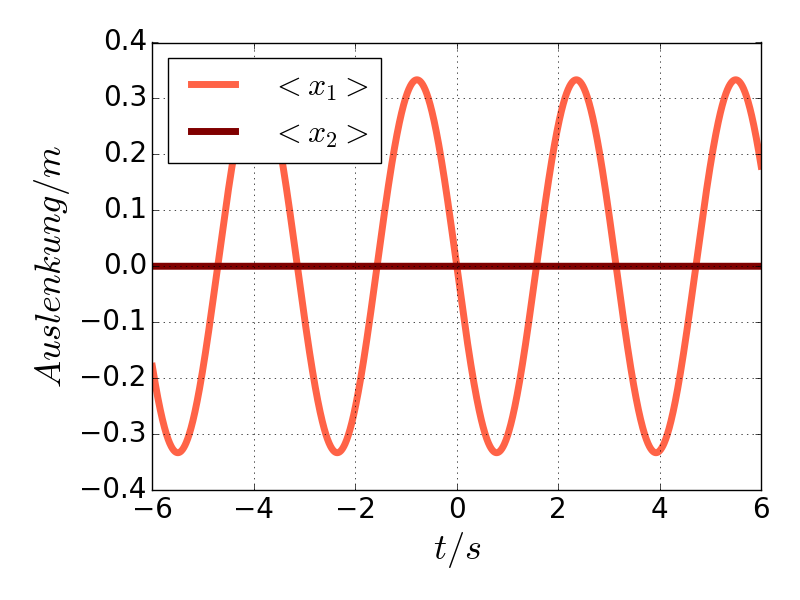
\includegraphics[width=\textwidth]{plots/<x2>nl0.png}
        \caption{$\kappa=0$.}
        \label{fig:x2_null}
      \end{subfigure}
      %\quad
      \begin{subfigure}[t]{0.5\textwidth}
          \centering
          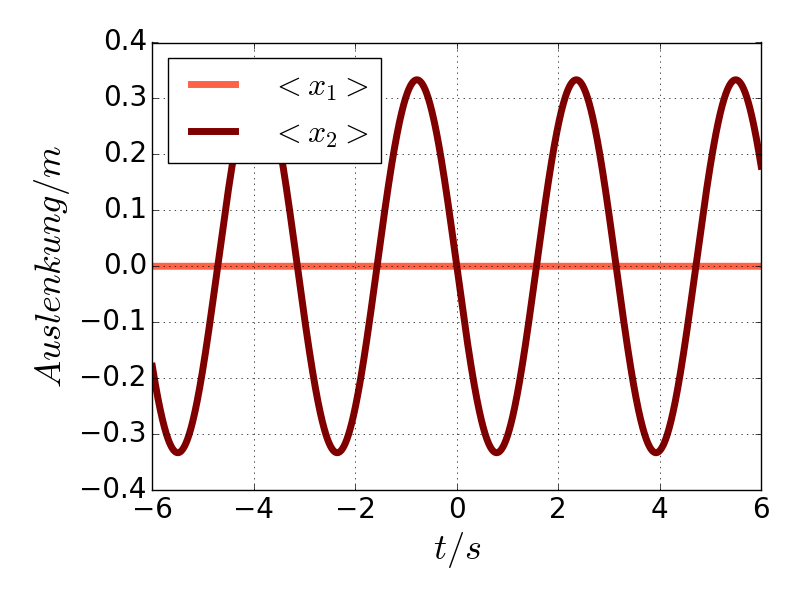
\includegraphics[width=\textwidth]{plots/<x1>nl0.png}
          \caption{$\kappa=\omega^2m-k=3$.}
          \label{fig:x1_null}
      \end{subfigure}
      %\quad
      \begin{subfigure}[t]{0.5\textwidth}
        \centering
        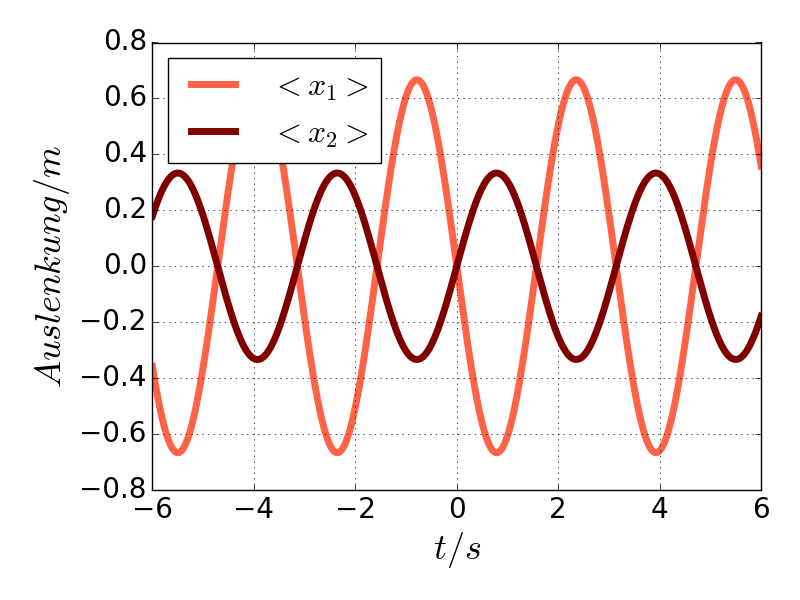
\includegraphics[width=\textwidth]{plots/<x12>nlschwach.png}
        \caption{$\kappa=1$.}
        \label{fig:schwach}
      \end{subfigure}
      %\quad
      \begin{subfigure}[t]{0.5\textwidth}sinusoidal
          \centering
          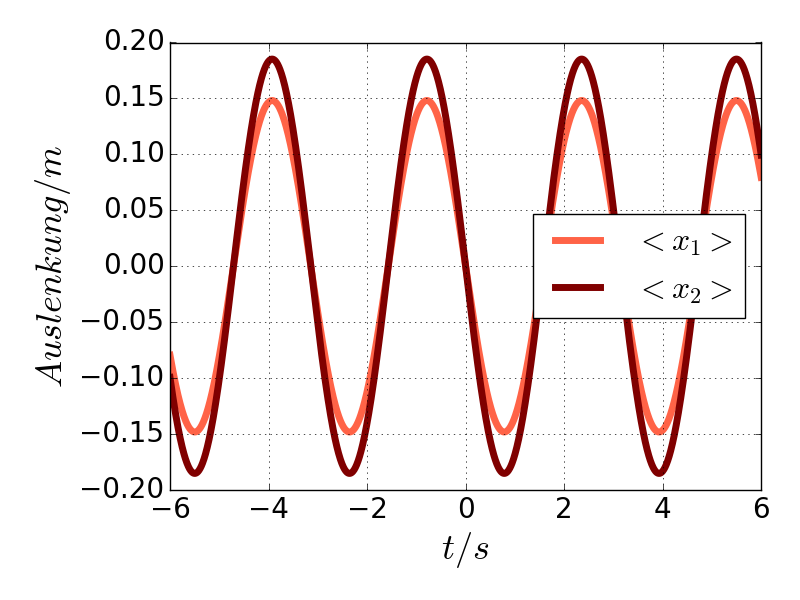
\includegraphics[width=\textwidth]{plots/<x12>nlstark.png}
          \caption{$\kappa=15$.}
          \label{fig:stark}
      \end{subfigure}
      %\quad
      \begin{subfigure}[t]{0.5\textwidth}
        \centering
        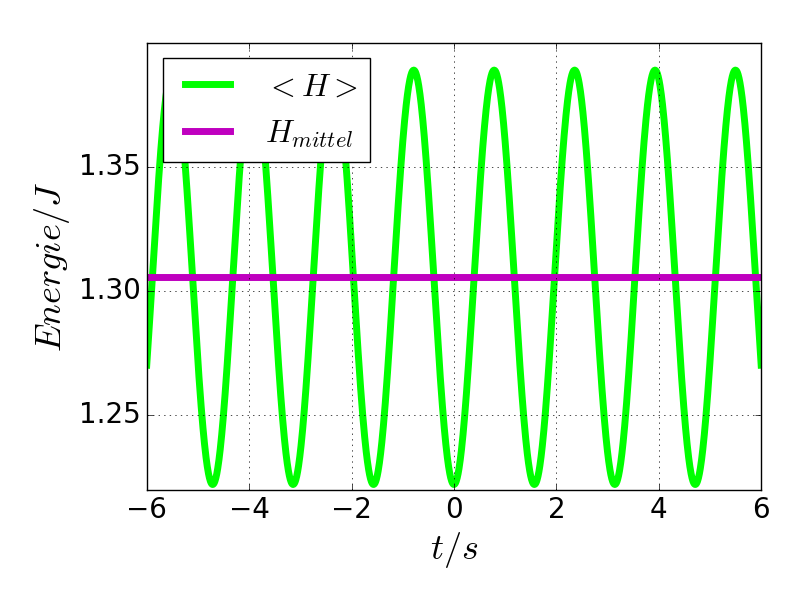
\includegraphics[width=\textwidth]{plots/<H>00_kappa0.png}
        \caption{$\kappa=0$.}
        \label{fig:H_kappa0}
      \end{subfigure}
      %\quad
      \begin{subfigure}[t]{0.5\textwidth}
          \centering
          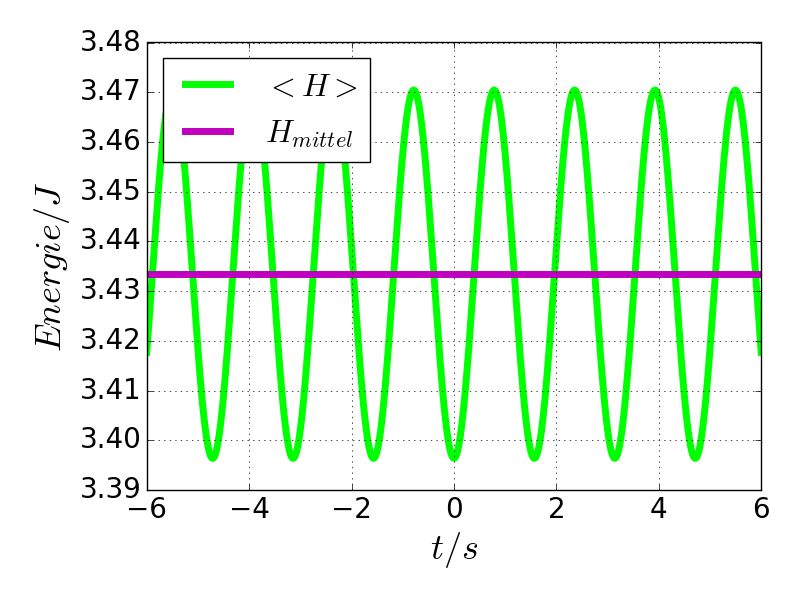
\includegraphics[width=\textwidth]{plots/<H>00_kappa15.png}
          \caption{$\kappa=15$.}
          \label{fig:H_kappa15}
      \end{subfigure}
      \caption{Erwartungswerte der gekoppelten Oszillatoren $\braket{x_1}_{n,l}$ und $\braket{x_2}_{n,l}$ für beliebigen Zustand $\Psi_{n,l}$, außerdem der Erwartungswert der Gesamtenergie $\braket{H(t)}_{0,0}$ und zeitliches Mittel $\overline{H}_{0,0}$ für den Grundzustand $\Psi_{0,0}$. Mit $\omega=2 , A=1 , k=1 , m=1 , \hbar=1$, für verschiedene Kopplungskonstanten $\kappa$.}
    \end{figure}
\fi

  \subsection{Zeitabhängige Erwartungswerte des Impulses}
    Die Transformation der Impulsoperatoren (\ref{koord_trafo_p}) hat die gleiche Form wie bei den Ortsoperatoren (\ref{koord_trafo_x}), die Berechnung der Erwartungswerte $\braket{p_{1 \atop 2}}_{n,l}$ und $\braket{p_{1\atop 2}^2}_{n,l}$ erfolgt darum analog, mit den Impuls-Erwartungswerten (\ref{erwartungswert_p_einzelner}) und (\ref{erwartungswert_p^2_einzelner}).
    Es gilt:
    \begin{align}
      \braket{p_{1 \atop 2}}_{n,l}=\frac{1}{\sqrt{2}}\left(\braket{p_+}_{n,l}\mp\braket{p_-}_{n,l}\right)
      =\frac{1}{\sqrt{2}}\left(\braket{p_+}_n^+\mp\braket{p_-}_l^-\right)
      =\frac{m}{\sqrt{2}}(\dot\zeta_+(t)\mp\dot\zeta_-(t)) \;
    \end{align}
    und
    \begin{align}
      \braket{p^2_{1\atop 2}}_{n,l}&=\frac{1}{2}\braket{(p_+\mp p_-)^2}_{n,l} \notag\\
      %=\frac{1}{2}\left(\braket{p_+^2}_n^+ \mp 2\braket{p_+}_n^+\braket{x_-}_l^- - \braket{x_-^2}_n^+\right) \notag\\
      &=\frac {m^2} 2 (\omega_+^2s_+^2(2n+1)+\dot\zeta_+^2(t) \mp 2\dot\zeta_+(t)\dot\zeta_-(t) + \omega_-^2s_-^2(2l+1)\dot\zeta_-^2(t)) \; .
    \end{align}
    Die Erwartungswerte sind ähnlich zu denen des Ortes.
    %Wie beim einzelnen Oszillator
    Es kommt nur ein Faktor hinzu und die $\zeta_\pm(t)$ werden zu ihren Ableitungen.

    Für eine Sinus-Treibkraft, sehen die Erwartungswerte fur $p_{1\atop 2}$ demnach so aus wie die $\braket{x_{1\atop 2}}_{n,l}$ nur mit skalierter Amplitude und phasenverschoben um $\pi$.
    Das Verhalten für die verschiedenen Kopplungskonstanten $\kappa$ ist ebenfalls identisch.

  \subsection{Erwartungswerte der Energie}
    Der zeitabhängige Erwartungswert $\braket{H(t)}_{n,l}$ des Hamilton-Operators für eine beliebige Treibkraft $S(t)$ ist auch mit dem Erwatungswert des einzelnen Oszillators berechenbar, indem wir wieder in den neuen Koordinaten arbeiten:
    \begin{align}
      \braket{H(t)}_{n,l} &= \braket{H_+(t)}_n^+ + \braket{H_-(t)}_l^- \notag\\
      &= E_{+,n}+E_{-,l} -L_+-L_- +m\dot\zeta_+^2(t)+m\dot\zeta_-^2(t) \; .
    \end{align}
    Der mittlere Erwartungswert $\overline{H}_{n,l}$ wird wieder in den neuen Koordinaten, mit Formel (\ref{mittleres_H}), berechnet.
    Weil die Quasienergien $\epsilon_{n,l}$ die Summe von $\epsilon_{+,n}$ und $\epsilon_{-,l}$ ist, kriegen wir sofort
    \begin{align}
      \overline{H}_{n,l}&=\overline{H}_{+,n}+\overline{H}_{-,l}  \notag\\
      &=E_{+,n}+E_{-,l} - \frac{\frac{1}{\sqrt 2} A}{4m(\omega_+^2-\omega^2)}\left(1-\frac{2\omega^2}{(\omega_+^2-\omega^2)}\right)
      - \frac{\frac{-1}{\sqrt 2} A}{4m(\omega_-^2-\omega^2)}\left(1-\frac{2\omega^2}{(\omega_-^2-\omega^2)}\right) \; .
    \end{align}

    \textbf{Sinusoidiale Treibkraft}

    Für das Beispiel der Sinus-Kraft folgt $\braket{H(t)}_{n,l}$ mit den ensprechenden Orts- und Impulserwartungswerten aus vorherigem Abschnitt und  $\overline{H}_{n,l}$ folgt aus Gleichung (\ref{mittleres_H}).
    Der Erwartungswert der Energie $\braket H_{0,0}$ und dessen zeitliches Mittel $\overline{H}(t)_{0,0}$ sind für die selben Konstanten wie zuvor
    \begin{equation}
      \omega=2 \;,\; A=1 \;,\; k=1 \;,\; m=1 \;,\; \hbar=1 \; ,
    \end{equation}
    in Abb.(\ref{ferg}) aufgetragen.
    Da beide Erwartungswerte wegen den $E_{+,n}/E_{-,l}$ abhängig von den Quantenzahlen sind, wird hier der einfachste Fall $n=l=0 \Rightarrow E_{\pm,0}=\hbar \omega_\pm/2$ betrachtet.
\iffalse
    \begin{figure}
      \begin{subfigure}[t]{0.5\textwidth}
        \centering
        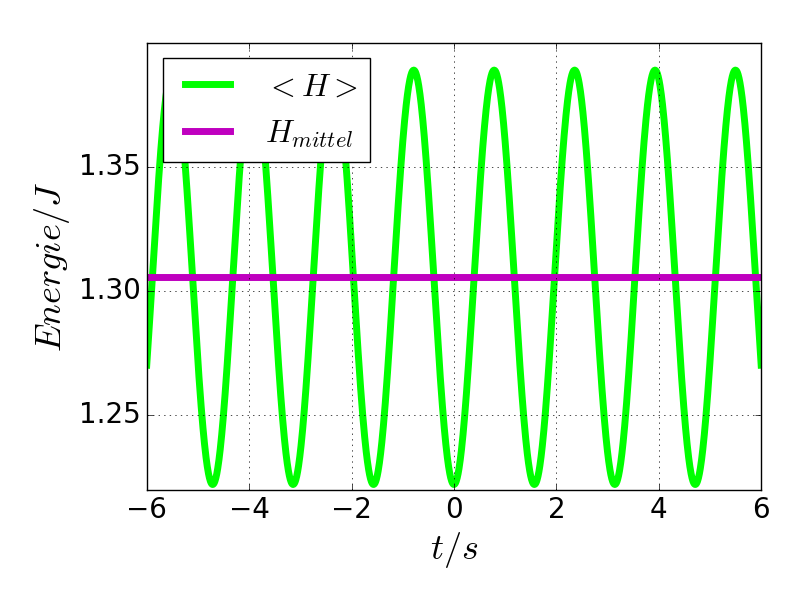
\includegraphics[width=\textwidth]{plots/<H>00_kappa0.png}
        \caption{$\kappa=0$.}
        \label{fig:H_kappa0}
      \end{subfigure}
      \quad
      \begin{subfigure}[t]{0.5\textwidth}
          \centering
          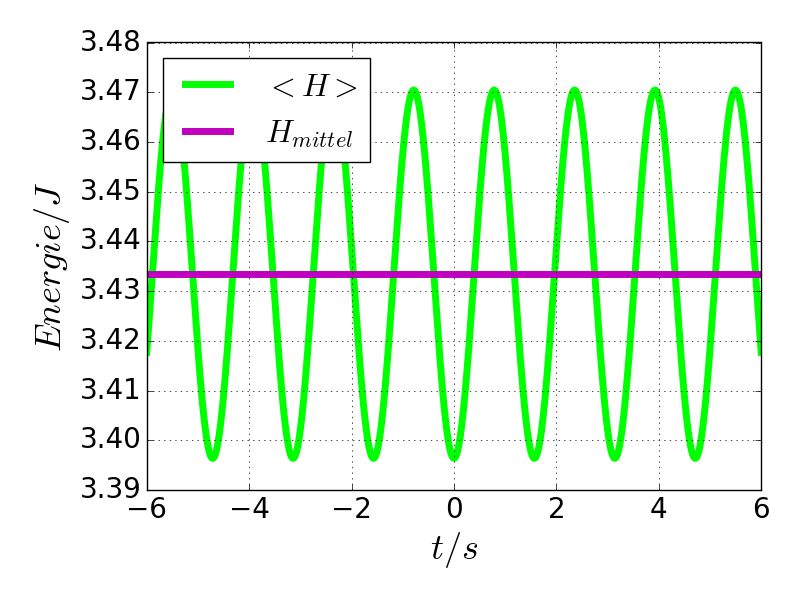
\includegraphics[width=\textwidth]{plots/<H>00_kappa15.png}
          \caption{$\kappa=15$.}
          \label{fig:H_kappa15}
      \end{subfigure}
      \caption{Erwartungswert der Gesamtenergie $\braket{H(t)}_{0,0}$ und zeitliches Mittel $\overline{H}_{0,0}$ für den Grundzustand $\Psi_{0,0}$ mit $\omega=2 \;,\; A=1 \;,\; k=1 \;,\; m=1 \;,\; \hbar=1$, für verschiedene Kopplungskonstanten $\kappa$.}
    \end{figure}
\fi
    Ohne Kopplung (\ref{fig:H_kappa0}) ist die mittlere Energie am geringsten, für eine möglichst starke/starre Kopplung (\ref{fig:H_kappa15}) wird die mittlere Energie im System maximal, weil die Treibkraft so möglichst viel Energie auf den angekoppelten Oszillator $x_2$ übetragen kann.
    \begin{figure}
      \begin{subfigure}[t]{0.5\textwidth}
        \centering
        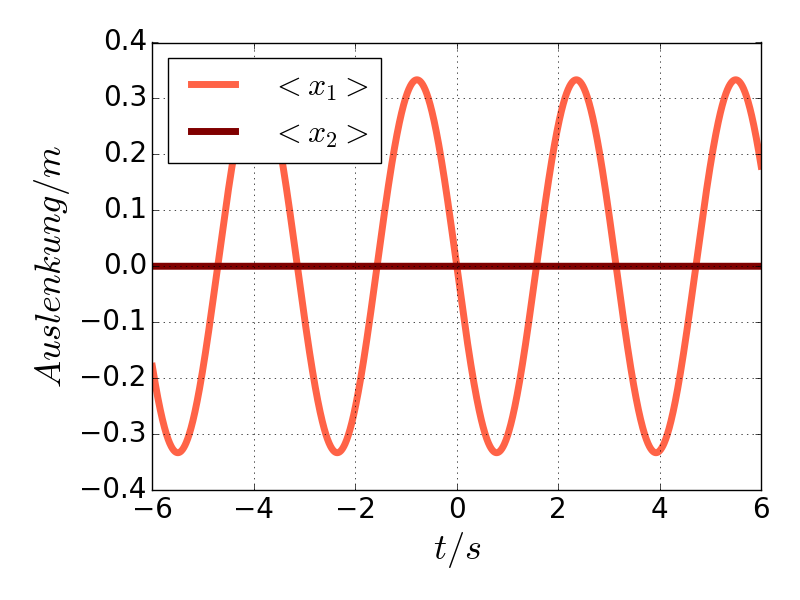
\includegraphics[width=\textwidth]{plots/<x2>nl0.png}
        \caption{$\kappa=0$.}
        \label{fig:x2_null}
      \end{subfigure}
      %\quad
      \begin{subfigure}[t]{0.5\textwidth}
          \centering
          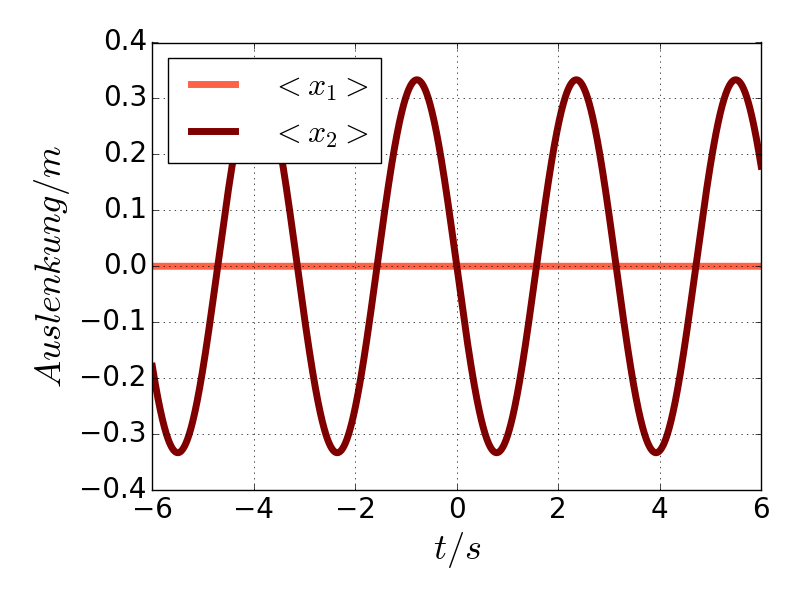
\includegraphics[width=\textwidth]{plots/<x1>nl0.png}
          \caption{$\kappa=\omega^2m-k=3$.}
          \label{fig:x1_null}
      \end{subfigure}
      %\quad
      \begin{subfigure}[t]{0.5\textwidth}
        \centering
        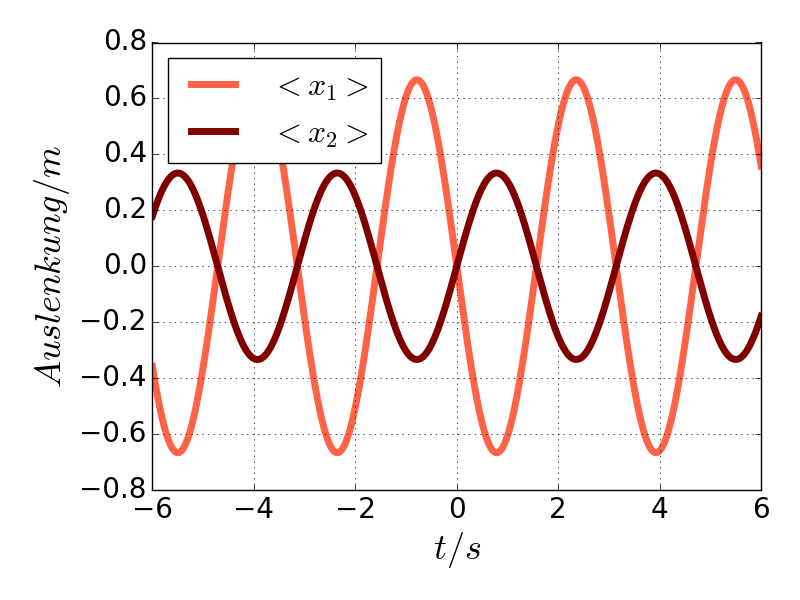
\includegraphics[width=\textwidth]{plots/<x12>nlschwach.png}
        \caption{$\kappa=1$.}
        \label{fig:schwach}
      \end{subfigure}
      %\quad
      \begin{subfigure}[t]{0.5\textwidth}
          \centering
          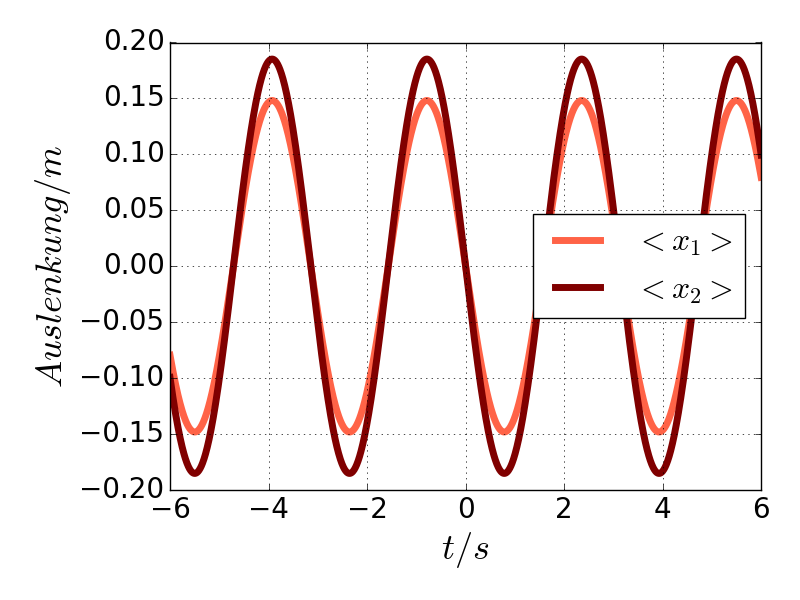
\includegraphics[width=\textwidth]{plots/<x12>nlstark.png}
          \caption{$\kappa=15$.}
          \label{fig:stark}
      \end{subfigure}
      %\quad
      \begin{subfigure}[t]{0.5\textwidth}
        \centering
        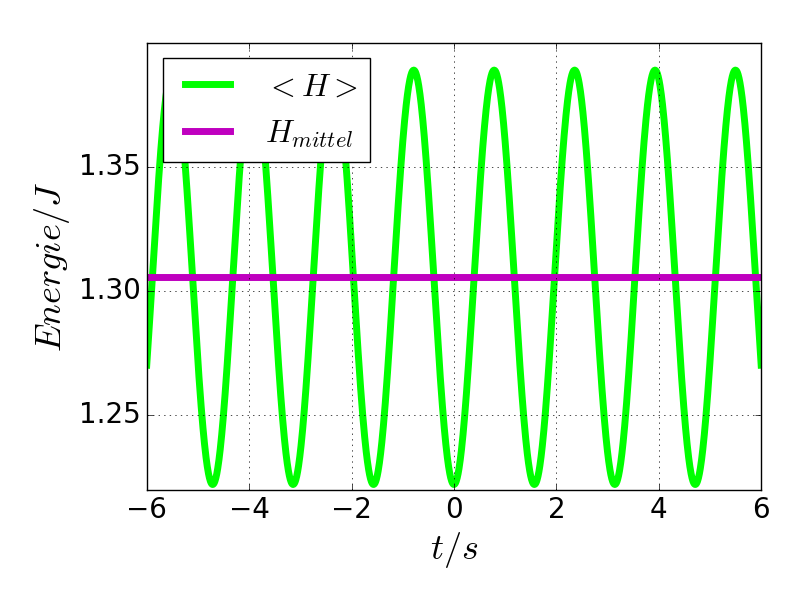
\includegraphics[width=\textwidth]{plots/<H>00_kappa0.png}
        \caption{$\kappa=0$.}
        \label{fig:H_kappa0}
      \end{subfigure}
      %\quad
      \begin{subfigure}[t]{0.5\textwidth}
          \centering
          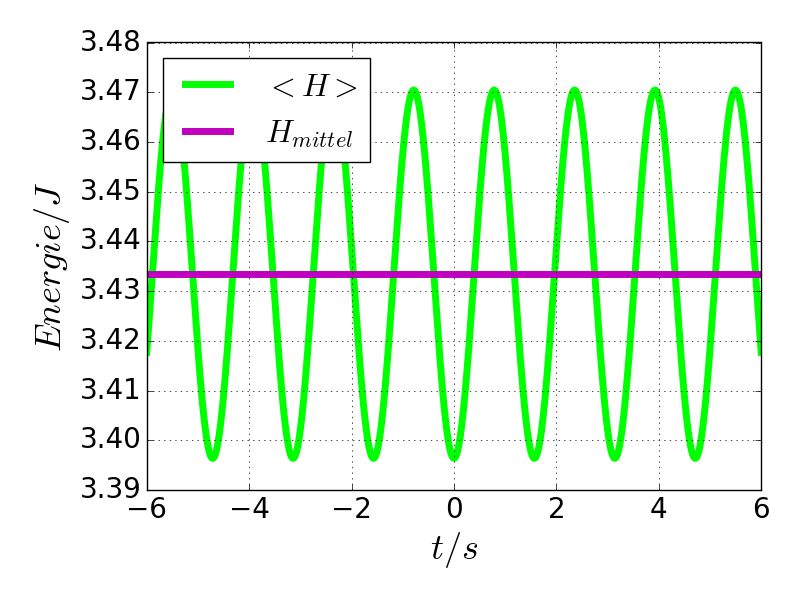
\includegraphics[width=\textwidth]{plots/<H>00_kappa15.png}
          \caption{$\kappa=15$.}
          \label{fig:H_kappa15}
      \end{subfigure}
      \caption{Erwartungswerte der gekoppelten Oszillatoren $\braket{x_1}_{n,l}$ und $\braket{x_2}_{n,l}$ für beliebigen Zustand $\Psi_{n,l}$, außerdem der Erwartungswert der Gesamtenergie $\braket{H(t)}_{0,0}$ und zeitliches Mittel $\overline{H}_{0,0}$ für den Grundzustand $\Psi_{0,0}$. Mit $\omega=2 \;,\; A=1 \;,\; k=1 \;,\; m=1 \;,\; \hbar=1$, für verschiedene Kopplungskonstanten $\kappa$.}
      \label{ferg}
    \end{figure}

\chapter{Zweite Quantisierung}

\chapter{Zusammenfassung und Ausblick}
\label{6}
In dieser Arbeit wurde das quantenmechanische Problem eines periodisch getriebenen harmonischen Oszillators näher betrachtet.
Nachdem die Floquet-Theorie in Grundzügen erklärt wurde, konnte das Floquet-Theorem anhand der Wellenfunktionen des getriebenen Oszillators verifiziert werden.
Mit einem Fourier-Reihen-Ansatz konnten die Quasienergien der Floquet-Theorie für eine beliebige periodische Treibkraft im System, in Abhängigkeit der Fourier-Koeffizienten der Kraft bestimmt werden.
Mit den Quasienergien kann unter anderem das zeitliche Mittel des Energie-Erwartungswertes berechnet werden, ohne diesen selbst zu kennen, wodurch ein einfacher erster Eindruck des Systems möglich ist.
Wir konnten z.\,B. frühzeitig feststellen, dass die Energie divergieren wird, wenn sich die Treibfrequenz nah der Oszillator-Eigenfrequenz befindet.

Nachdem die Erwartungswerte für den Ort, den Impuls und die Energie berechnet wurden, haben wir das System um einen weiteren angekoppelten Oszillator erweitert.
Die Lösung der Schrödinger-Gleichung gelang hier mit einer Koordinatentransformation, welche den Hamilton-Operator in eine Summe aus zwei unabhängigen Hamilton-Operatoren überführte.
Damit wussten wir, dass die Lösung durch ein Produkt der Wellenfunktionen in den neuen Koordinaten gegeben ist, was für beliebig viele Hamilton-Operatoren ebenso korrekt ist.
Die Form der Koordinaten-Transformation kann hierbei aus den klassischen Normalmoden gewonnen werden, welche wiederum durch das Diagonalisieren einer Matrix bei der Lösung des klassichen Problems erhalten werden.
Dies sollte ebenso für beliebig viele gekoppelte Oszillatoren funktionieren, womit die Wellenfunktionen für ein System aus $n$ gekoppelten Oszillatoren genauso aufgestellt werden können.
Für ungleiche Massen und Potentialkonstanten ergeben sich im Allgemeinen aber kompliziertere Normalmoden und Transformationen.

Für die zwei gekoppelten getriebenen Oszillatoren haben wir, unter Ausnutzung der neuen Variablen und der Erwartungswerte des einzelnen Oszillators, ebenfalls die Erwartungswerte berechnet und zudem visualisiert.
Es ergab sich an vielen Stellen ein Verhalten der Erwartungswerte, welches dem des klassischen Systems entspricht.

Zum Schluss der Arbeit wurde ein weiteres Mal der einzelne getriebene Oszillator behandelt.
Diesmal wurde das Problem in der 2. Quantisierung betrachtet.
Mit einem geeigneten Ansatz, welchen wir anhand der Lösung in Ortsdarstellung motiviert haben, haben wir das darstellungsunabhängige Wellenfunktion-Ket aufstellen können.
In der 2. Quantisierung haben wir damit die gleichen Erwartungswerte wie in der Ortsdarstellung erhalten.
Um mehrere gekoppelte Oszillatoren in der Besetzungszahldarstellung zu betrachten, können die gleichen Transformationen für die Operatoren gewählt werden wie zuvor in der Ortsdarstellung.
Weil die Operatoren beim Wellenfunktion-Ket nur im Exponenten vorkommen, führt dies sofort auf die Produktform.
%Der Pduktansatz funktioniert für beliebig viele unabhängige Operatoren.
%Die Koordinatentranformation


\appendix
% Hier beginnt der Anhang, nummeriert in lateinischen Buchstaben
\chapter{Ein Anhangskapitel}

Hier könnte ein Anhang stehen, falls Sie z.B. Code, Konstruktionszeichnungen oder Ähnliches mit in die Arbeit bringen wollen. Im Normalfall stehen jedoch alle Ihre Resultate im Hauptteil der Bachelorarbeit und ein Anhang ist überflüssig.


\backmatter
\printbibliography

\cleardoublepage
\thispagestyle{empty}
\section*{Eidesstattliche Versicherung}
Ich versichere hiermit an Eides statt, dass ich die vorliegende Abschlussarbeit mit dem Titel \enquote{\thetitle} selbstständig und ohne unzulässige fremde Hilfe erbracht habe.
Ich habe keine anderen als die angegebenen Quellen und Hilfsmittel benutzt, sowie wörtliche und sinngemäße Zitate kenntlich gemacht. 
Die Arbeit hat in gleicher oder ähnlicher Form noch keiner Prüfungsbehörde vorgelegen.

\vspace*{1cm}\noindent
\begin{center}
  \begin{tabular}{@{}p{0.4\textwidth}@{\hspace{0.15\textwidth}}p{0.4\textwidth}@{}}
  \rule{\linewidth}{0.25pt}& \rule{\linewidth}{0.25pt}\\
  Ort, Datum & Unterschrift
  \end{tabular}
\end{center}

\subsection*{Belehrung}
Wer vorsätzlich gegen eine die Täuschung über Prüfungsleistungen betreffende Regelung einer Hochschulprüfungsordnung verstößt, handelt ordnungswidrig.
Die Ordnungswidrigkeit kann mit einer Geldbuße von bis zu \SI[round-mode=places, round-precision=2]{50000}{€} geahndet werden. 
Zuständige Verwaltungsbehörde für die Verfolgung und Ahndung von Ordnungswidrigkeiten ist der Kanzler/die Kanzlerin der Technischen Universität Dortmund. 
Im Falle eines mehrfachen oder sonstigen schwerwiegenden Täuschungsversuches kann der Prüfling zudem exmatrikuliert werden \mbox{(\S\,63 Abs. 5 Hochschulgesetz --HG--).}

Die Abgabe einer falschen Versicherung an Eides statt wird mit Freiheitsstrafe bis zu 3 Jahren oder mit Geldstrafe bestraft.

Die Technische Universität Dortmund wird ggf.\ elektronische Vergleichswerkzeuge (wie z.\,B.\ die Software \enquote{turnitin}) zur Überprüfung von Ordnungswidrigkeiten in Prüfungsverfahren nutzen. \\[\baselineskip]

\noindent Die oben stehende Belehrung habe ich zur Kenntnis genommen.\\[1cm]
\begin{center}
\begin{tabular}{@{}p{0.4\textwidth}@{\hspace{0.15\textwidth}}p{0.4\textwidth}@{}}
\rule{\linewidth}{0.25pt}& \rule{\linewidth}{0.25pt}\\
Ort, Datum & Unterschrift
\end{tabular}
\end{center}

\end{document}
